\documentclass[twoside]{book}

% Packages required by doxygen
\usepackage{fixltx2e}
\usepackage{calc}
\usepackage{doxygen}
\usepackage[export]{adjustbox} % also loads graphicx
\usepackage{graphicx}
\usepackage[utf8]{inputenc}
\usepackage{makeidx}
\usepackage{multicol}
\usepackage{multirow}
\PassOptionsToPackage{warn}{textcomp}
\usepackage{textcomp}
\usepackage[nointegrals]{wasysym}
\usepackage[table]{xcolor}

% Font selection
\usepackage[T1]{fontenc}
\usepackage[scaled=.90]{helvet}
\usepackage{courier}
\usepackage{amssymb}
\usepackage{sectsty}
\renewcommand{\familydefault}{\sfdefault}
\allsectionsfont{%
  \fontseries{bc}\selectfont%
  \color{darkgray}%
}
\renewcommand{\DoxyLabelFont}{%
  \fontseries{bc}\selectfont%
  \color{darkgray}%
}
\newcommand{\+}{\discretionary{\mbox{\scriptsize$\hookleftarrow$}}{}{}}

% Page & text layout
\usepackage{geometry}
\geometry{%
  a4paper,%
  top=2.5cm,%
  bottom=2.5cm,%
  left=2.5cm,%
  right=2.5cm%
}
\tolerance=750
\hfuzz=15pt
\hbadness=750
\setlength{\emergencystretch}{15pt}
\setlength{\parindent}{0cm}
\setlength{\parskip}{3ex plus 2ex minus 2ex}
\makeatletter
\renewcommand{\paragraph}{%
  \@startsection{paragraph}{4}{0ex}{-1.0ex}{1.0ex}{%
    \normalfont\normalsize\bfseries\SS@parafont%
  }%
}
\renewcommand{\subparagraph}{%
  \@startsection{subparagraph}{5}{0ex}{-1.0ex}{1.0ex}{%
    \normalfont\normalsize\bfseries\SS@subparafont%
  }%
}
\makeatother

% Headers & footers
\usepackage{fancyhdr}
\pagestyle{fancyplain}
\fancyhead[LE]{\fancyplain{}{\bfseries\thepage}}
\fancyhead[CE]{\fancyplain{}{}}
\fancyhead[RE]{\fancyplain{}{\bfseries\leftmark}}
\fancyhead[LO]{\fancyplain{}{\bfseries\rightmark}}
\fancyhead[CO]{\fancyplain{}{}}
\fancyhead[RO]{\fancyplain{}{\bfseries\thepage}}
\fancyfoot[LE]{\fancyplain{}{}}
\fancyfoot[CE]{\fancyplain{}{}}
\fancyfoot[RE]{\fancyplain{}{\bfseries\scriptsize Generated by Doxygen }}
\fancyfoot[LO]{\fancyplain{}{\bfseries\scriptsize Generated by Doxygen }}
\fancyfoot[CO]{\fancyplain{}{}}
\fancyfoot[RO]{\fancyplain{}{}}
\renewcommand{\footrulewidth}{0.4pt}
\renewcommand{\chaptermark}[1]{%
  \markboth{#1}{}%
}
\renewcommand{\sectionmark}[1]{%
  \markright{\thesection\ #1}%
}

% Indices & bibliography
\usepackage{natbib}
\usepackage[titles]{tocloft}
\setcounter{tocdepth}{3}
\setcounter{secnumdepth}{5}
\makeindex

% Hyperlinks (required, but should be loaded last)
\usepackage{ifpdf}
\ifpdf
  \usepackage[pdftex,pagebackref=true]{hyperref}
\else
  \usepackage[ps2pdf,pagebackref=true]{hyperref}
\fi
\hypersetup{%
  colorlinks=true,%
  linkcolor=blue,%
  citecolor=blue,%
  unicode%
}

% Custom commands
\newcommand{\clearemptydoublepage}{%
  \newpage{\pagestyle{empty}\cleardoublepage}%
}

\usepackage{caption}
\captionsetup{labelsep=space,justification=centering,font={bf},singlelinecheck=off,skip=4pt,position=top}

%===== C O N T E N T S =====

\begin{document}

% Titlepage & ToC
\hypersetup{pageanchor=false,
             bookmarksnumbered=true,
             pdfencoding=unicode
            }
\pagenumbering{alph}
\begin{titlepage}
\vspace*{7cm}
\begin{center}%
{\Large Pogodynka\+\_\+w57003 }\\
\vspace*{1cm}
{\large Generated by Doxygen 1.8.14}\\
\end{center}
\end{titlepage}
\clearemptydoublepage
\pagenumbering{roman}
\tableofcontents
\clearemptydoublepage
\pagenumbering{arabic}
\hypersetup{pageanchor=true}

%--- Begin generated contents ---
\chapter{Namespace Index}
\section{Packages}
Here are the packages with brief descriptions (if available)\+:\begin{DoxyCompactList}
\item\contentsline{section}{\mbox{\hyperlink{namespace_pogodynka__w57003}{Pogodynka\+\_\+w57003}} \\*Głowna funkcjonalność progamu }{\pageref{namespace_pogodynka__w57003}}{}
\end{DoxyCompactList}

\chapter{Hierarchical Index}
\section{Class Hierarchy}
This inheritance list is sorted roughly, but not completely, alphabetically\+:\begin{DoxyCompactList}
\item \contentsline{section}{Pogodynka\+\_\+w57003.\+city}{\pageref{class_pogodynka__w57003_1_1city}}{}
\item \contentsline{section}{Pogodynka\+\_\+w57003.\+Weather\+Info.\+coord}{\pageref{class_pogodynka__w57003_1_1_weather_info_1_1coord}}{}
\item Form\begin{DoxyCompactList}
\item \contentsline{section}{Pogodynka\+\_\+w57003.\+panel\+\_\+glony}{\pageref{class_pogodynka__w57003_1_1panel__glony}}{}
\end{DoxyCompactList}
\item \contentsline{section}{Pogodynka\+\_\+w57003.\+list}{\pageref{class_pogodynka__w57003_1_1list}}{}
\item \contentsline{section}{Pogodynka\+\_\+w57003.\+main}{\pageref{class_pogodynka__w57003_1_1main}}{}
\item \contentsline{section}{Pogodynka\+\_\+w57003.\+Weather\+Info.\+main}{\pageref{class_pogodynka__w57003_1_1_weather_info_1_1main}}{}
\item \contentsline{section}{Pogodynka\+\_\+w57003.\+Program}{\pageref{class_pogodynka__w57003_1_1_program}}{}
\item \contentsline{section}{Pogodynka\+\_\+w57003.\+Weather\+Info.\+Root}{\pageref{class_pogodynka__w57003_1_1_weather_info_1_1_root}}{}
\item \contentsline{section}{Pogodynka\+\_\+w57003.\+Weather\+Info.\+sys}{\pageref{class_pogodynka__w57003_1_1_weather_info_1_1sys}}{}
\item \contentsline{section}{Pogodynka\+\_\+w57003.\+Weather\+Info.\+weather}{\pageref{class_pogodynka__w57003_1_1_weather_info_1_1weather}}{}
\item \contentsline{section}{Pogodynka\+\_\+w57003.\+weather}{\pageref{class_pogodynka__w57003_1_1weather}}{}
\item \contentsline{section}{Pogodynka\+\_\+w57003.\+weather\+Forcast}{\pageref{class_pogodynka__w57003_1_1weather_forcast}}{}
\item \contentsline{section}{Pogodynka\+\_\+w57003.\+Weather\+Info}{\pageref{class_pogodynka__w57003_1_1_weather_info}}{}
\item \contentsline{section}{Pogodynka\+\_\+w57003.\+Weather\+Info.\+wind}{\pageref{class_pogodynka__w57003_1_1_weather_info_1_1wind}}{}
\item \contentsline{section}{Pogodynka\+\_\+w57003.\+wind}{\pageref{class_pogodynka__w57003_1_1wind}}{}
\end{DoxyCompactList}

\chapter{Class Index}
\section{Class List}
Here are the classes, structs, unions and interfaces with brief descriptions\+:\begin{DoxyCompactList}
\item\contentsline{section}{\mbox{\hyperlink{class_pogodynka__w57003_1_1city}{Pogodynka\+\_\+w57003.\+city}} }{\pageref{class_pogodynka__w57003_1_1city}}{}
\item\contentsline{section}{\mbox{\hyperlink{class_pogodynka__w57003_1_1_weather_info_1_1coord}{Pogodynka\+\_\+w57003.\+Weather\+Info.\+coord}} }{\pageref{class_pogodynka__w57003_1_1_weather_info_1_1coord}}{}
\item\contentsline{section}{\mbox{\hyperlink{class_pogodynka__w57003_1_1list}{Pogodynka\+\_\+w57003.\+list}} }{\pageref{class_pogodynka__w57003_1_1list}}{}
\item\contentsline{section}{\mbox{\hyperlink{class_pogodynka__w57003_1_1main}{Pogodynka\+\_\+w57003.\+main}} }{\pageref{class_pogodynka__w57003_1_1main}}{}
\item\contentsline{section}{\mbox{\hyperlink{class_pogodynka__w57003_1_1_weather_info_1_1main}{Pogodynka\+\_\+w57003.\+Weather\+Info.\+main}} }{\pageref{class_pogodynka__w57003_1_1_weather_info_1_1main}}{}
\item\contentsline{section}{\mbox{\hyperlink{class_pogodynka__w57003_1_1panel__glony}{Pogodynka\+\_\+w57003.\+panel\+\_\+glony}} }{\pageref{class_pogodynka__w57003_1_1panel__glony}}{}
\item\contentsline{section}{\mbox{\hyperlink{class_pogodynka__w57003_1_1_program}{Pogodynka\+\_\+w57003.\+Program}} }{\pageref{class_pogodynka__w57003_1_1_program}}{}
\item\contentsline{section}{\mbox{\hyperlink{class_pogodynka__w57003_1_1_weather_info_1_1_root}{Pogodynka\+\_\+w57003.\+Weather\+Info.\+Root}} }{\pageref{class_pogodynka__w57003_1_1_weather_info_1_1_root}}{}
\item\contentsline{section}{\mbox{\hyperlink{class_pogodynka__w57003_1_1_weather_info_1_1sys}{Pogodynka\+\_\+w57003.\+Weather\+Info.\+sys}} }{\pageref{class_pogodynka__w57003_1_1_weather_info_1_1sys}}{}
\item\contentsline{section}{\mbox{\hyperlink{class_pogodynka__w57003_1_1_weather_info_1_1weather}{Pogodynka\+\_\+w57003.\+Weather\+Info.\+weather}} }{\pageref{class_pogodynka__w57003_1_1_weather_info_1_1weather}}{}
\item\contentsline{section}{\mbox{\hyperlink{class_pogodynka__w57003_1_1weather}{Pogodynka\+\_\+w57003.\+weather}} }{\pageref{class_pogodynka__w57003_1_1weather}}{}
\item\contentsline{section}{\mbox{\hyperlink{class_pogodynka__w57003_1_1weather_forcast}{Pogodynka\+\_\+w57003.\+weather\+Forcast}} }{\pageref{class_pogodynka__w57003_1_1weather_forcast}}{}
\item\contentsline{section}{\mbox{\hyperlink{class_pogodynka__w57003_1_1_weather_info}{Pogodynka\+\_\+w57003.\+Weather\+Info}} }{\pageref{class_pogodynka__w57003_1_1_weather_info}}{}
\item\contentsline{section}{\mbox{\hyperlink{class_pogodynka__w57003_1_1_weather_info_1_1wind}{Pogodynka\+\_\+w57003.\+Weather\+Info.\+wind}} }{\pageref{class_pogodynka__w57003_1_1_weather_info_1_1wind}}{}
\item\contentsline{section}{\mbox{\hyperlink{class_pogodynka__w57003_1_1wind}{Pogodynka\+\_\+w57003.\+wind}} }{\pageref{class_pogodynka__w57003_1_1wind}}{}
\end{DoxyCompactList}

\chapter{Namespace Documentation}
\hypertarget{namespace_pogodynka__w57003}{}\section{Pogodynka\+\_\+w57003 Namespace Reference}
\label{namespace_pogodynka__w57003}\index{Pogodynka\+\_\+w57003@{Pogodynka\+\_\+w57003}}


Głowna funkcjonalność progamu  


\subsection*{Classes}
\begin{DoxyCompactItemize}
\item 
class \mbox{\hyperlink{class_pogodynka__w57003_1_1city}{city}}
\item 
class \mbox{\hyperlink{class_pogodynka__w57003_1_1list}{list}}
\item 
class \mbox{\hyperlink{class_pogodynka__w57003_1_1main}{main}}
\item 
class \mbox{\hyperlink{class_pogodynka__w57003_1_1panel__glony}{panel\+\_\+glony}}
\item 
class \mbox{\hyperlink{class_pogodynka__w57003_1_1_program}{Program}}
\item 
class \mbox{\hyperlink{class_pogodynka__w57003_1_1weather}{weather}}
\item 
class \mbox{\hyperlink{class_pogodynka__w57003_1_1weather_forcast}{weather\+Forcast}}
\item 
class \mbox{\hyperlink{class_pogodynka__w57003_1_1_weather_info}{Weather\+Info}}
\item 
class \mbox{\hyperlink{class_pogodynka__w57003_1_1wind}{wind}}
\end{DoxyCompactItemize}


\subsection{Detailed Description}
Głowna funkcjonalność progamu 

Klasa dla pogody oaktualnej 

Klasa dla prognozy pogody 
\chapter{Class Documentation}
\hypertarget{class_pogodynka__w57003_1_1city}{}\section{Pogodynka\+\_\+w57003.\+city Class Reference}
\label{class_pogodynka__w57003_1_1city}\index{Pogodynka\+\_\+w57003.\+city@{Pogodynka\+\_\+w57003.\+city}}
\subsection*{Properties}
\begin{DoxyCompactItemize}
\item 
\mbox{\Hypertarget{class_pogodynka__w57003_1_1city_a160a2b22892d59b257efb2b7eb135f9b}\label{class_pogodynka__w57003_1_1city_a160a2b22892d59b257efb2b7eb135f9b}} 
string {\bfseries name}\hspace{0.3cm}{\ttfamily  \mbox{[}get, set\mbox{]}}
\end{DoxyCompactItemize}


The documentation for this class was generated from the following file\+:\begin{DoxyCompactItemize}
\item 
C\+:/\+Users/\+Paweł/\+Documents/\+Visual Studio 2015/\+Projects/\+Pogodynka\+\_\+w57003/\+Pogodynka\+\_\+w57003/weather\+Forcast.\+cs\end{DoxyCompactItemize}

\hypertarget{class_pogodynka__w57003_1_1_weather_info_1_1coord}{}\section{Pogodynka\+\_\+w57003.\+Weather\+Info.\+coord Class Reference}
\label{class_pogodynka__w57003_1_1_weather_info_1_1coord}\index{Pogodynka\+\_\+w57003.\+Weather\+Info.\+coord@{Pogodynka\+\_\+w57003.\+Weather\+Info.\+coord}}


klasa odpowiedzialna za pozycję geograficzną miejscowości  


\subsection*{Properties}
\begin{DoxyCompactItemize}
\item 
\mbox{\Hypertarget{class_pogodynka__w57003_1_1_weather_info_1_1coord_a6dc94b6e0c88eee7dacdf38e8e502fcb}\label{class_pogodynka__w57003_1_1_weather_info_1_1coord_a6dc94b6e0c88eee7dacdf38e8e502fcb}} 
double {\bfseries lon}\hspace{0.3cm}{\ttfamily  \mbox{[}get, set\mbox{]}}
\item 
\mbox{\Hypertarget{class_pogodynka__w57003_1_1_weather_info_1_1coord_af187780c76202970c1efc4f0c010d0fe}\label{class_pogodynka__w57003_1_1_weather_info_1_1coord_af187780c76202970c1efc4f0c010d0fe}} 
double {\bfseries lat}\hspace{0.3cm}{\ttfamily  \mbox{[}get, set\mbox{]}}
\end{DoxyCompactItemize}


\subsection{Detailed Description}
klasa odpowiedzialna za pozycję geograficzną miejscowości 



The documentation for this class was generated from the following file\+:\begin{DoxyCompactItemize}
\item 
C\+:/\+Users/\+Paweł/\+Documents/\+Visual Studio 2015/\+Projects/\+Pogodynka\+\_\+w57003/\+Pogodynka\+\_\+w57003/weather\+Info.\+cs\end{DoxyCompactItemize}

\hypertarget{class_pogodynka__w57003_1_1list}{}\section{Pogodynka\+\_\+w57003.\+list Class Reference}
\label{class_pogodynka__w57003_1_1list}\index{Pogodynka\+\_\+w57003.\+list@{Pogodynka\+\_\+w57003.\+list}}
\subsection*{Properties}
\begin{DoxyCompactItemize}
\item 
\mbox{\Hypertarget{class_pogodynka__w57003_1_1list_ae9b9dcbb2a0d9f5dd950bc0f013327c5}\label{class_pogodynka__w57003_1_1list_ae9b9dcbb2a0d9f5dd950bc0f013327c5}} 
string {\bfseries dt\+\_\+txt}\hspace{0.3cm}{\ttfamily  \mbox{[}get, set\mbox{]}}
\item 
\mbox{\Hypertarget{class_pogodynka__w57003_1_1list_aa9e8fb1a4f3ed369b3873e3a0fa09357}\label{class_pogodynka__w57003_1_1list_aa9e8fb1a4f3ed369b3873e3a0fa09357}} 
\mbox{\hyperlink{class_pogodynka__w57003_1_1wind}{wind}} {\bfseries wind}\hspace{0.3cm}{\ttfamily  \mbox{[}get, set\mbox{]}}
\item 
\mbox{\Hypertarget{class_pogodynka__w57003_1_1list_a022a0fd0e9b0dd60f302dcdfa1a80ae9}\label{class_pogodynka__w57003_1_1list_a022a0fd0e9b0dd60f302dcdfa1a80ae9}} 
\mbox{\hyperlink{class_pogodynka__w57003_1_1main}{main}} {\bfseries main}\hspace{0.3cm}{\ttfamily  \mbox{[}get, set\mbox{]}}
\item 
\mbox{\Hypertarget{class_pogodynka__w57003_1_1list_aab12839c65ae24bf60f65b092210b5a4}\label{class_pogodynka__w57003_1_1list_aab12839c65ae24bf60f65b092210b5a4}} 
List$<$ \mbox{\hyperlink{class_pogodynka__w57003_1_1weather}{weather}} $>$ {\bfseries weather}\hspace{0.3cm}{\ttfamily  \mbox{[}get, set\mbox{]}}
\end{DoxyCompactItemize}


The documentation for this class was generated from the following file\+:\begin{DoxyCompactItemize}
\item 
C\+:/\+Users/\+Paweł/\+Documents/\+Visual Studio 2015/\+Projects/\+Pogodynka\+\_\+w57003/\+Pogodynka\+\_\+w57003/weather\+Forcast.\+cs\end{DoxyCompactItemize}

\hypertarget{class_pogodynka__w57003_1_1main}{}\section{Pogodynka\+\_\+w57003.\+main Class Reference}
\label{class_pogodynka__w57003_1_1main}\index{Pogodynka\+\_\+w57003.\+main@{Pogodynka\+\_\+w57003.\+main}}


klasa odpowiedzialna za pobranie informacji o temperaturze, ciśnieniu, oraz wilgotności powietrza  


\subsection*{Properties}
\begin{DoxyCompactItemize}
\item 
\mbox{\Hypertarget{class_pogodynka__w57003_1_1main_a17f39b6d6da5d6d247bcd4d209b4f226}\label{class_pogodynka__w57003_1_1main_a17f39b6d6da5d6d247bcd4d209b4f226}} 
double {\bfseries temp}\hspace{0.3cm}{\ttfamily  \mbox{[}get, set\mbox{]}}
\item 
\mbox{\Hypertarget{class_pogodynka__w57003_1_1main_a252f264966164ce699bf14ef40309ba5}\label{class_pogodynka__w57003_1_1main_a252f264966164ce699bf14ef40309ba5}} 
double {\bfseries pressure}\hspace{0.3cm}{\ttfamily  \mbox{[}get, set\mbox{]}}
\item 
\mbox{\Hypertarget{class_pogodynka__w57003_1_1main_abc8be82c5bb42bc5442b75aeed0926bb}\label{class_pogodynka__w57003_1_1main_abc8be82c5bb42bc5442b75aeed0926bb}} 
double {\bfseries humidity}\hspace{0.3cm}{\ttfamily  \mbox{[}get, set\mbox{]}}
\end{DoxyCompactItemize}


\subsection{Detailed Description}
klasa odpowiedzialna za pobranie informacji o temperaturze, ciśnieniu, oraz wilgotności powietrza 



The documentation for this class was generated from the following file\+:\begin{DoxyCompactItemize}
\item 
C\+:/\+Users/\+Paweł/\+Documents/\+Visual Studio 2015/\+Projects/\+Pogodynka\+\_\+w57003/\+Pogodynka\+\_\+w57003/weather\+Forcast.\+cs\end{DoxyCompactItemize}

\hypertarget{class_pogodynka__w57003_1_1_weather_info_1_1main}{}\section{Pogodynka\+\_\+w57003.\+Weather\+Info.\+main Class Reference}
\label{class_pogodynka__w57003_1_1_weather_info_1_1main}\index{Pogodynka\+\_\+w57003.\+Weather\+Info.\+main@{Pogodynka\+\_\+w57003.\+Weather\+Info.\+main}}


klasa odpowiedzialalna za pobraine informacji o temepraturze, ciśnieniu, oraz wilgotności  


\subsection*{Properties}
\begin{DoxyCompactItemize}
\item 
\mbox{\Hypertarget{class_pogodynka__w57003_1_1_weather_info_1_1main_a5120c22c35a0da4b5eb20aa939885211}\label{class_pogodynka__w57003_1_1_weather_info_1_1main_a5120c22c35a0da4b5eb20aa939885211}} 
double {\bfseries temp}\hspace{0.3cm}{\ttfamily  \mbox{[}get, set\mbox{]}}
\item 
\mbox{\Hypertarget{class_pogodynka__w57003_1_1_weather_info_1_1main_acdf846f787b99c43f66eaaa2a0ce01ce}\label{class_pogodynka__w57003_1_1_weather_info_1_1main_acdf846f787b99c43f66eaaa2a0ce01ce}} 
double {\bfseries pressure}\hspace{0.3cm}{\ttfamily  \mbox{[}get, set\mbox{]}}
\item 
\mbox{\Hypertarget{class_pogodynka__w57003_1_1_weather_info_1_1main_a73edaa1d4e96d6d43e82ab379eceaac5}\label{class_pogodynka__w57003_1_1_weather_info_1_1main_a73edaa1d4e96d6d43e82ab379eceaac5}} 
double {\bfseries humidity}\hspace{0.3cm}{\ttfamily  \mbox{[}get, set\mbox{]}}
\end{DoxyCompactItemize}


\subsection{Detailed Description}
klasa odpowiedzialalna za pobraine informacji o temepraturze, ciśnieniu, oraz wilgotności 



The documentation for this class was generated from the following file\+:\begin{DoxyCompactItemize}
\item 
C\+:/\+Users/\+Paweł/\+Documents/\+Visual Studio 2015/\+Projects/\+Pogodynka\+\_\+w57003/\+Pogodynka\+\_\+w57003/weather\+Info.\+cs\end{DoxyCompactItemize}

\hypertarget{class_pogodynka__w57003_1_1panel__glony}{}\section{Pogodynka\+\_\+w57003.\+panel\+\_\+glony Class Reference}
\label{class_pogodynka__w57003_1_1panel__glony}\index{Pogodynka\+\_\+w57003.\+panel\+\_\+glony@{Pogodynka\+\_\+w57003.\+panel\+\_\+glony}}
Inheritance diagram for Pogodynka\+\_\+w57003.\+panel\+\_\+glony\+:\begin{figure}[H]
\begin{center}
\leavevmode
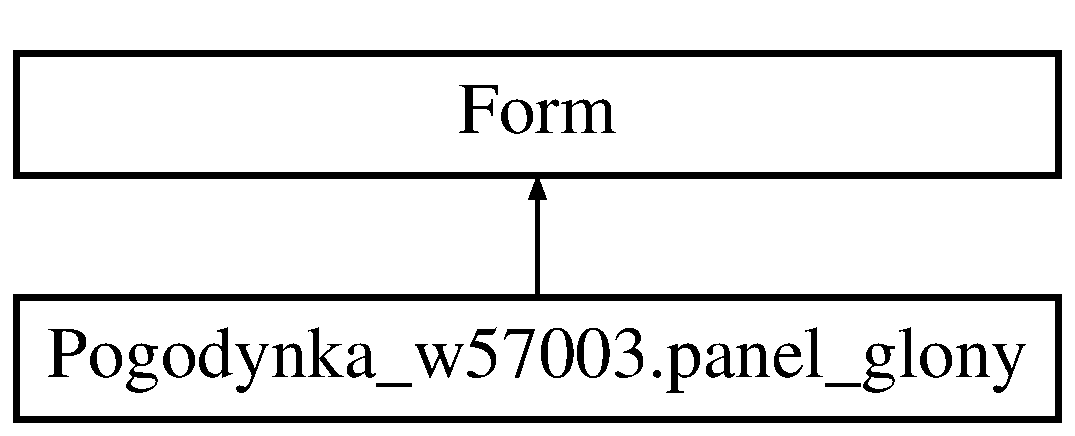
\includegraphics[height=2.000000cm]{class_pogodynka__w57003_1_1panel__glony}
\end{center}
\end{figure}
\subsection*{Public Member Functions}
\begin{DoxyCompactItemize}
\item 
\mbox{\hyperlink{class_pogodynka__w57003_1_1panel__glony_a5722f839e53134d3fd67f320dec8056e}{panel\+\_\+glony}} ()
\begin{DoxyCompactList}\small\item\em Domyślne miasto wczytywane przy starcie programu \end{DoxyCompactList}\end{DoxyCompactItemize}
\subsection*{Protected Member Functions}
\begin{DoxyCompactItemize}
\item 
override void \mbox{\hyperlink{class_pogodynka__w57003_1_1panel__glony_af7cfae8068adcc3589d5b990b982e226}{Dispose}} (bool disposing)
\begin{DoxyCompactList}\small\item\em Clean up any resources being used. \end{DoxyCompactList}\end{DoxyCompactItemize}
\subsection*{Private Member Functions}
\begin{DoxyCompactItemize}
\item 
void \mbox{\hyperlink{class_pogodynka__w57003_1_1panel__glony_a1b552bb32257c708d4c7755b60cb54a0}{get\+Weather}} (string \mbox{\hyperlink{class_pogodynka__w57003_1_1city}{city}})
\begin{DoxyCompactList}\small\item\em Funkcjonalność pobrania danych z A\+PI dla pogody aktualnej \end{DoxyCompactList}\item 
void \mbox{\hyperlink{class_pogodynka__w57003_1_1panel__glony_aa08ea57aa456c27766dcb8d032478d4b}{get\+Forcast}} (string \mbox{\hyperlink{class_pogodynka__w57003_1_1city}{city}})
\begin{DoxyCompactList}\small\item\em Funkcjonalność pobrania danych z A\+PI dla prognozy pogody \end{DoxyCompactList}\item 
Image \mbox{\hyperlink{class_pogodynka__w57003_1_1panel__glony_a92d766dd29d34e246e2e99deb2591b82}{set\+Icon}} (string icon\+ID)
\begin{DoxyCompactList}\small\item\em Klasa pobierająca obrazek przedstawiający stan nieba \end{DoxyCompactList}\item 
\mbox{\Hypertarget{class_pogodynka__w57003_1_1panel__glony_aaf474a16b7accdb4f5fba157d91d7286}\label{class_pogodynka__w57003_1_1panel__glony_aaf474a16b7accdb4f5fba157d91d7286}} 
void {\bfseries background\+Worker3\+\_\+\+Do\+Work} (object sender, Do\+Work\+Event\+Args e)
\item 
void \mbox{\hyperlink{class_pogodynka__w57003_1_1panel__glony_ad2d405552ab48f25e21c26c78cb660b4}{schowajelementydocka}} ()
\begin{DoxyCompactList}\small\item\em Klasa chowająca kontrolki w docku \end{DoxyCompactList}\item 
void \mbox{\hyperlink{class_pogodynka__w57003_1_1panel__glony_a40e7412c72125b4544218fb03a4af1d3}{pokazelementydocka}} ()
\begin{DoxyCompactList}\small\item\em Klasa Pokazjuąca kontrolki w docku \end{DoxyCompactList}\item 
void \mbox{\hyperlink{class_pogodynka__w57003_1_1panel__glony_ab0736937098fec29cd5311a389c2b0b4}{picture\+Box6\+\_\+\+Click}} (object sender, Event\+Args e)
\begin{DoxyCompactList}\small\item\em Funkcjonalnośc przyciska menu wysuwający i chowający banner \end{DoxyCompactList}\item 
void \mbox{\hyperlink{class_pogodynka__w57003_1_1panel__glony_a7947ac67ced4aa22c0f52aed6ad3b3f3}{strona\+\_\+glowna\+\_\+\+Link\+Clicked}} (object sender, Link\+Label\+Link\+Clicked\+Event\+Args e)
\begin{DoxyCompactList}\small\item\em Funckjonalnośc kontrolki Strona głowna \end{DoxyCompactList}\item 
void \mbox{\hyperlink{class_pogodynka__w57003_1_1panel__glony_ac5516e612d6350c23e9caaa4682dcfa7}{Mapy\+\_\+experta\+\_\+\+Link\+Clicked}} (object sender, Link\+Label\+Link\+Clicked\+Event\+Args e)
\begin{DoxyCompactList}\small\item\em Funckjonalnośc kontrolki Mapy eksperta \end{DoxyCompactList}\item 
void \mbox{\hyperlink{class_pogodynka__w57003_1_1panel__glony_ac3892cf16a3589e5578defe1786710e0}{Wyszukiwarka\+\_\+\+Link\+Clicked\+\_\+1}} (object sender, Link\+Label\+Link\+Clicked\+Event\+Args e)
\begin{DoxyCompactList}\small\item\em Funckjonalnośc kontrolki wyszukiwarka \end{DoxyCompactList}\item 
void \mbox{\hyperlink{class_pogodynka__w57003_1_1panel__glony_a8d32fcf8f9a2d131dc124427170bc84c}{Zamknij\+\_\+\+Link\+Clicked\+\_\+1}} (object sender, Link\+Label\+Link\+Clicked\+Event\+Args e)
\begin{DoxyCompactList}\small\item\em Funkcjonalnoś przyciska zamknij \end{DoxyCompactList}\item 
void \mbox{\hyperlink{class_pogodynka__w57003_1_1panel__glony_aa677678689be30d9ddab7cc4de694bf0}{estofex\+\_\+\+Link\+Clicked\+\_\+1}} (object sender, Link\+Label\+Link\+Clicked\+Event\+Args e)
\begin{DoxyCompactList}\small\item\em Funckjonalnośc kontrolki estofex w panelu mapy eksperta \end{DoxyCompactList}\item 
void \mbox{\hyperlink{class_pogodynka__w57003_1_1panel__glony_ac50b569c9ce770f430f4d644bc758d51}{um\+\_\+\+Link\+Clicked\+\_\+1}} (object sender, Link\+Label\+Link\+Clicked\+Event\+Args e)
\begin{DoxyCompactList}\small\item\em Funckjonalnośc kontrolki mapy um w panelu mapy eksperta \end{DoxyCompactList}\item 
\mbox{\Hypertarget{class_pogodynka__w57003_1_1panel__glony_a1fbfdc80359bf8836628c39abc48ec14}\label{class_pogodynka__w57003_1_1panel__glony_a1fbfdc80359bf8836628c39abc48ec14}} 
void {\bfseries label12\+\_\+\+Click} (object sender, Event\+Args e)
\item 
\mbox{\Hypertarget{class_pogodynka__w57003_1_1panel__glony_a818f89ab7880da12e9bab877186c43ea}\label{class_pogodynka__w57003_1_1panel__glony_a818f89ab7880da12e9bab877186c43ea}} 
void {\bfseries label12\+\_\+\+Click\+\_\+1} (object sender, Event\+Args e)
\item 
void \mbox{\hyperlink{class_pogodynka__w57003_1_1panel__glony_a58881a0fcdaac088f2ba3108cd62db63}{showcityum}} ()
\begin{DoxyCompactList}\small\item\em Funkcja pkazująca mista po wybraniu kontrolki Model UM \end{DoxyCompactList}\item 
void \mbox{\hyperlink{class_pogodynka__w57003_1_1panel__glony_a0548ec7f9130fc67e27ad426e0cb79da}{hidecityum}} ()
\begin{DoxyCompactList}\small\item\em Funkcja ukeywająca mista po wybraniu kontrolki Model UM \end{DoxyCompactList}\item 
void \mbox{\hyperlink{class_pogodynka__w57003_1_1panel__glony_af58e72c559c60a71a859212c03f33f69}{set\+Modelm}} (int row, int col)
\begin{DoxyCompactList}\small\item\em Funkcja implmentująca szerokośc i długośc geograficzną okreslonego miasta \end{DoxyCompactList}\item 
void \mbox{\hyperlink{class_pogodynka__w57003_1_1panel__glony_a75827f3c30a1c8dc76f94ff41e1427dc}{Bliaystok\+\_\+\+Click\+\_\+1}} (object sender, Event\+Args e)
\begin{DoxyCompactList}\small\item\em metody przypisujące wspólrzędne po kliknięciu na miasta \end{DoxyCompactList}\item 
\mbox{\Hypertarget{class_pogodynka__w57003_1_1panel__glony_a548ec312f7b53b05c6f772495f043022}\label{class_pogodynka__w57003_1_1panel__glony_a548ec312f7b53b05c6f772495f043022}} 
void {\bfseries bydgoszcz\+\_\+\+Click\+\_\+1} (object sender, Event\+Args e)
\item 
\mbox{\Hypertarget{class_pogodynka__w57003_1_1panel__glony_a02669c1228d1c82352f1a3c512354eb2}\label{class_pogodynka__w57003_1_1panel__glony_a02669c1228d1c82352f1a3c512354eb2}} 
void {\bfseries gdansk\+\_\+\+Click\+\_\+1} (object sender, Event\+Args e)
\item 
\mbox{\Hypertarget{class_pogodynka__w57003_1_1panel__glony_a738d6c1be023e9404ab7e1a9158507a5}\label{class_pogodynka__w57003_1_1panel__glony_a738d6c1be023e9404ab7e1a9158507a5}} 
void {\bfseries gorzow\+\_\+wlkp\+\_\+\+Click\+\_\+1} (object sender, Event\+Args e)
\item 
\mbox{\Hypertarget{class_pogodynka__w57003_1_1panel__glony_a64bd15aed857996f9a6bbd0fae4f3ab0}\label{class_pogodynka__w57003_1_1panel__glony_a64bd15aed857996f9a6bbd0fae4f3ab0}} 
void {\bfseries katowice\+\_\+\+Click\+\_\+1} (object sender, Event\+Args e)
\item 
\mbox{\Hypertarget{class_pogodynka__w57003_1_1panel__glony_a585bf9de909a3374009339c5edeaab15}\label{class_pogodynka__w57003_1_1panel__glony_a585bf9de909a3374009339c5edeaab15}} 
void {\bfseries kielce\+\_\+\+Click\+\_\+1} (object sender, Event\+Args e)
\item 
\mbox{\Hypertarget{class_pogodynka__w57003_1_1panel__glony_aada40ed519215c55fbb12b3be5a2ef49}\label{class_pogodynka__w57003_1_1panel__glony_aada40ed519215c55fbb12b3be5a2ef49}} 
void {\bfseries krakow\+\_\+\+Click\+\_\+1} (object sender, Event\+Args e)
\item 
\mbox{\Hypertarget{class_pogodynka__w57003_1_1panel__glony_a53d5ff19d844dd236ce0ba69205e193d}\label{class_pogodynka__w57003_1_1panel__glony_a53d5ff19d844dd236ce0ba69205e193d}} 
void {\bfseries lublin\+\_\+\+Click\+\_\+1} (object sender, Event\+Args e)
\item 
\mbox{\Hypertarget{class_pogodynka__w57003_1_1panel__glony_a566f50415d7a7575e91e669b8ba1bd0a}\label{class_pogodynka__w57003_1_1panel__glony_a566f50415d7a7575e91e669b8ba1bd0a}} 
void {\bfseries lodz\+\_\+\+Click\+\_\+1} (object sender, Event\+Args e)
\item 
\mbox{\Hypertarget{class_pogodynka__w57003_1_1panel__glony_afa95f5557b54d6cd6b275b5e3fd7cb3a}\label{class_pogodynka__w57003_1_1panel__glony_afa95f5557b54d6cd6b275b5e3fd7cb3a}} 
void {\bfseries panel\+\_\+mapyexperta\+\_\+\+Paint} (object sender, Paint\+Event\+Args e)
\item 
\mbox{\Hypertarget{class_pogodynka__w57003_1_1panel__glony_a55a3b0dcd51dee1edbf2df9a859ba618}\label{class_pogodynka__w57003_1_1panel__glony_a55a3b0dcd51dee1edbf2df9a859ba618}} 
void {\bfseries opole\+\_\+\+Click\+\_\+1} (object sender, Event\+Args e)
\item 
\mbox{\Hypertarget{class_pogodynka__w57003_1_1panel__glony_add0774db536fafe4bfa643348f0bc9f7}\label{class_pogodynka__w57003_1_1panel__glony_add0774db536fafe4bfa643348f0bc9f7}} 
void {\bfseries poznan\+\_\+\+Click\+\_\+1} (object sender, Event\+Args e)
\item 
\mbox{\Hypertarget{class_pogodynka__w57003_1_1panel__glony_a8122958c5546eb29466354cd9990aa58}\label{class_pogodynka__w57003_1_1panel__glony_a8122958c5546eb29466354cd9990aa58}} 
void {\bfseries rzeszow\+\_\+\+Click\+\_\+1} (object sender, Event\+Args e)
\item 
\mbox{\Hypertarget{class_pogodynka__w57003_1_1panel__glony_a0918ba7669b7ae735e4fb147c86a8b64}\label{class_pogodynka__w57003_1_1panel__glony_a0918ba7669b7ae735e4fb147c86a8b64}} 
void {\bfseries szczecin\+\_\+\+Click\+\_\+1} (object sender, Event\+Args e)
\item 
\mbox{\Hypertarget{class_pogodynka__w57003_1_1panel__glony_a2228ed471be507c408e5e2569e06d6da}\label{class_pogodynka__w57003_1_1panel__glony_a2228ed471be507c408e5e2569e06d6da}} 
void {\bfseries torun\+\_\+\+Click\+\_\+1} (object sender, Event\+Args e)
\item 
\mbox{\Hypertarget{class_pogodynka__w57003_1_1panel__glony_a5b129569bb213ebfafc9548b97c7296b}\label{class_pogodynka__w57003_1_1panel__glony_a5b129569bb213ebfafc9548b97c7296b}} 
void {\bfseries warszawa\+\_\+\+Click\+\_\+1} (object sender, Event\+Args e)
\item 
\mbox{\Hypertarget{class_pogodynka__w57003_1_1panel__glony_a801fa394be306a6759ff0a4f96b9e636}\label{class_pogodynka__w57003_1_1panel__glony_a801fa394be306a6759ff0a4f96b9e636}} 
void {\bfseries wroclaw\+\_\+\+Click\+\_\+1} (object sender, Event\+Args e)
\item 
\mbox{\Hypertarget{class_pogodynka__w57003_1_1panel__glony_a77c9805cfc1044e4b9912b2deb139028}\label{class_pogodynka__w57003_1_1panel__glony_a77c9805cfc1044e4b9912b2deb139028}} 
void \mbox{\hyperlink{class_pogodynka__w57003_1_1panel__glony_a77c9805cfc1044e4b9912b2deb139028}{zielona\+\_\+gora\+\_\+\+Click\+\_\+1}} (object sender, Event\+Args e)
\begin{DoxyCompactList}\small\item\em /summary$>$ \end{DoxyCompactList}\item 
void \mbox{\hyperlink{class_pogodynka__w57003_1_1panel__glony_ae9fe7cb3a32f5d4c437ab29212d6ea42}{Legenda\+\_\+\+Click\+\_\+1}} (object sender, Event\+Args e)
\begin{DoxyCompactList}\small\item\em funkcjonalnośc kontrolk legenda \end{DoxyCompactList}\item 
void \mbox{\hyperlink{class_pogodynka__w57003_1_1panel__glony_a0ecf75f825f5031f164a81ea0e61de1c}{button\+\_\+search\+\_\+\+Click\+\_\+1}} (object sender, Event\+Args e)
\begin{DoxyCompactList}\small\item\em Funkcjonalnosc przycisku \char`\"{}\+Wyszukaj\char`\"{} ,oraz metody pobierające tekst z pola tekstowego \end{DoxyCompactList}\item 
void \mbox{\hyperlink{class_pogodynka__w57003_1_1panel__glony_af5137f1d9cbd6b2de8018a922c8eb87b}{Mapa\+\_\+burzowa\+\_\+\+Link\+Clicked\+\_\+1}} (object sender, Link\+Label\+Link\+Clicked\+Event\+Args e)
\begin{DoxyCompactList}\small\item\em Funckjonalnośc kontrolki Mapa burzowa w panelu mapy eksperta \end{DoxyCompactList}\item 
\mbox{\Hypertarget{class_pogodynka__w57003_1_1panel__glony_a51f8b1e9e647f9e3c549383b28d3c545}\label{class_pogodynka__w57003_1_1panel__glony_a51f8b1e9e647f9e3c549383b28d3c545}} 
void {\bfseries Form1\+\_\+\+Load} (object sender, Event\+Args e)
\item 
\mbox{\Hypertarget{class_pogodynka__w57003_1_1panel__glony_a6167e1624375f77ff4533b1e7f961edc}\label{class_pogodynka__w57003_1_1panel__glony_a6167e1624375f77ff4533b1e7f961edc}} 
void {\bfseries label1\+\_\+\+Click} (object sender, Event\+Args e)
\item 
\mbox{\Hypertarget{class_pogodynka__w57003_1_1panel__glony_afc8dc7c22b9481f62a650f08e5798fed}\label{class_pogodynka__w57003_1_1panel__glony_afc8dc7c22b9481f62a650f08e5798fed}} 
void {\bfseries label3\+\_\+\+Click} (object sender, Event\+Args e)
\item 
\mbox{\Hypertarget{class_pogodynka__w57003_1_1panel__glony_a6c721469331c8eaf0d4a7de4d8f7acfe}\label{class_pogodynka__w57003_1_1panel__glony_a6c721469331c8eaf0d4a7de4d8f7acfe}} 
void {\bfseries picture\+Box1\+\_\+\+Click} (object sender, Event\+Args e)
\item 
\mbox{\Hypertarget{class_pogodynka__w57003_1_1panel__glony_a5b28280fad60a92dd50f8afd7fdf090d}\label{class_pogodynka__w57003_1_1panel__glony_a5b28280fad60a92dd50f8afd7fdf090d}} 
void {\bfseries panel4\+\_\+\+Paint} (object sender, Paint\+Event\+Args e)
\item 
\mbox{\Hypertarget{class_pogodynka__w57003_1_1panel__glony_a1f498dbb0ba257e63334a0d87cb72f79}\label{class_pogodynka__w57003_1_1panel__glony_a1f498dbb0ba257e63334a0d87cb72f79}} 
void {\bfseries label1\+\_\+\+Click\+\_\+1} (object sender, Event\+Args e)
\item 
\mbox{\Hypertarget{class_pogodynka__w57003_1_1panel__glony_ad5bd9cb20a1da128d7619ece256bf1da}\label{class_pogodynka__w57003_1_1panel__glony_ad5bd9cb20a1da128d7619ece256bf1da}} 
void {\bfseries label10\+\_\+\+Click} (object sender, Event\+Args e)
\item 
\mbox{\Hypertarget{class_pogodynka__w57003_1_1panel__glony_a512774a6ab3e7e1623c74b06142ea0f3}\label{class_pogodynka__w57003_1_1panel__glony_a512774a6ab3e7e1623c74b06142ea0f3}} 
void {\bfseries picture\+Url\+\_\+\+Click} (object sender, Event\+Args e)
\item 
\mbox{\Hypertarget{class_pogodynka__w57003_1_1panel__glony_a01e97cdfb5fcadcdf709d4055c9aa565}\label{class_pogodynka__w57003_1_1panel__glony_a01e97cdfb5fcadcdf709d4055c9aa565}} 
void {\bfseries link\+Label1\+\_\+\+Link\+Clicked} (object sender, Link\+Label\+Link\+Clicked\+Event\+Args e)
\item 
void \mbox{\hyperlink{class_pogodynka__w57003_1_1panel__glony_a611ee70952200993f8066c71042452de}{Initialize\+Component}} ()
\begin{DoxyCompactList}\small\item\em Required method for Designer support -\/ do not modify the contents of this method with the code editor. \end{DoxyCompactList}\end{DoxyCompactItemize}
\subsection*{Private Attributes}
\begin{DoxyCompactItemize}
\item 
const string \mbox{\hyperlink{class_pogodynka__w57003_1_1panel__glony_a66dfd1c1fa2fc6daa20d17f8bf64c7a4}{A\+P\+P\+ID}} = \char`\"{}5018a726f091f2f233b3af11f9e207c8\char`\"{}
\begin{DoxyCompactList}\small\item\em Klucz A\+PI pobrane z witryny openweather.\+org \end{DoxyCompactList}\item 
System.\+Component\+Model.\+I\+Container \mbox{\hyperlink{class_pogodynka__w57003_1_1panel__glony_aa887be71e8f5b4267c82225f05b88ae2}{components}} = null
\begin{DoxyCompactList}\small\item\em Required designer variable. \end{DoxyCompactList}\item 
\mbox{\Hypertarget{class_pogodynka__w57003_1_1panel__glony_a8e714ed561f0833133090c8e94e8d2c0}\label{class_pogodynka__w57003_1_1panel__glony_a8e714ed561f0833133090c8e94e8d2c0}} 
System.\+Windows.\+Forms.\+Label {\bfseries label\+\_\+city}
\item 
\mbox{\Hypertarget{class_pogodynka__w57003_1_1panel__glony_a4e6b70274b747f25558c77c9f3773ec0}\label{class_pogodynka__w57003_1_1panel__glony_a4e6b70274b747f25558c77c9f3773ec0}} 
System.\+Windows.\+Forms.\+Label {\bfseries label\+\_\+country}
\item 
\mbox{\Hypertarget{class_pogodynka__w57003_1_1panel__glony_abacfb365dfa726f0c10afbbf70ac434d}\label{class_pogodynka__w57003_1_1panel__glony_abacfb365dfa726f0c10afbbf70ac434d}} 
System.\+Windows.\+Forms.\+Image\+List {\bfseries image\+List1}
\item 
\mbox{\Hypertarget{class_pogodynka__w57003_1_1panel__glony_a16f73538b1eac666c53797dcb4e5c9c5}\label{class_pogodynka__w57003_1_1panel__glony_a16f73538b1eac666c53797dcb4e5c9c5}} 
System.\+Windows.\+Forms.\+Picture\+Box {\bfseries picture\+Box1}
\item 
\mbox{\Hypertarget{class_pogodynka__w57003_1_1panel__glony_a3b75d6990cdb369eee1e8b58b0f6c3d6}\label{class_pogodynka__w57003_1_1panel__glony_a3b75d6990cdb369eee1e8b58b0f6c3d6}} 
System.\+Windows.\+Forms.\+Picture\+Box {\bfseries picture\+Box2}
\item 
\mbox{\Hypertarget{class_pogodynka__w57003_1_1panel__glony_a91d81a76eb1b0311c69f6af39e433387}\label{class_pogodynka__w57003_1_1panel__glony_a91d81a76eb1b0311c69f6af39e433387}} 
System.\+Windows.\+Forms.\+Label {\bfseries label\+\_\+day\+\_\+forcast}
\item 
\mbox{\Hypertarget{class_pogodynka__w57003_1_1panel__glony_a78e63c3bc774c34731a6c686ae04d37b}\label{class_pogodynka__w57003_1_1panel__glony_a78e63c3bc774c34731a6c686ae04d37b}} 
System.\+Windows.\+Forms.\+Label {\bfseries label\+\_\+conditionals\+\_\+forcast}
\item 
\mbox{\Hypertarget{class_pogodynka__w57003_1_1panel__glony_a7620ba32225d2b0ad545af3738564e2c}\label{class_pogodynka__w57003_1_1panel__glony_a7620ba32225d2b0ad545af3738564e2c}} 
System.\+Windows.\+Forms.\+Label {\bfseries label\+\_\+preesure\+\_\+forcast}
\item 
\mbox{\Hypertarget{class_pogodynka__w57003_1_1panel__glony_ad8a6982ab27582aacd69efdc75f763ec}\label{class_pogodynka__w57003_1_1panel__glony_ad8a6982ab27582aacd69efdc75f763ec}} 
System.\+Windows.\+Forms.\+Label {\bfseries label\+\_\+wind\+\_\+forcast}
\item 
\mbox{\Hypertarget{class_pogodynka__w57003_1_1panel__glony_a8dbf994aeef45fc28561ceb827f0ce69}\label{class_pogodynka__w57003_1_1panel__glony_a8dbf994aeef45fc28561ceb827f0ce69}} 
System.\+Windows.\+Forms.\+Label {\bfseries label\+\_\+forcast}
\item 
\mbox{\Hypertarget{class_pogodynka__w57003_1_1panel__glony_a8a122c44cabb0ad9fb6e91d4fe712c6a}\label{class_pogodynka__w57003_1_1panel__glony_a8a122c44cabb0ad9fb6e91d4fe712c6a}} 
System.\+Windows.\+Forms.\+Label {\bfseries label\+\_\+day\+\_\+forcast2}
\item 
\mbox{\Hypertarget{class_pogodynka__w57003_1_1panel__glony_a7a1066a568f5522b57e6324a048883bc}\label{class_pogodynka__w57003_1_1panel__glony_a7a1066a568f5522b57e6324a048883bc}} 
System.\+Windows.\+Forms.\+Label {\bfseries label\+\_\+conditionals\+\_\+forcast2}
\item 
\mbox{\Hypertarget{class_pogodynka__w57003_1_1panel__glony_a8cde67f766b24f62c8c4b42369ff2917}\label{class_pogodynka__w57003_1_1panel__glony_a8cde67f766b24f62c8c4b42369ff2917}} 
System.\+Windows.\+Forms.\+Label {\bfseries label\+\_\+pressure\+\_\+forcast2}
\item 
\mbox{\Hypertarget{class_pogodynka__w57003_1_1panel__glony_aef67dde1d2d88770e02067565058d836}\label{class_pogodynka__w57003_1_1panel__glony_aef67dde1d2d88770e02067565058d836}} 
System.\+Windows.\+Forms.\+Label {\bfseries label\+\_\+wind\+\_\+forcast2}
\item 
\mbox{\Hypertarget{class_pogodynka__w57003_1_1panel__glony_a2c07c51a616478cd8fab540fe0debf15}\label{class_pogodynka__w57003_1_1panel__glony_a2c07c51a616478cd8fab540fe0debf15}} 
System.\+Windows.\+Forms.\+Label {\bfseries label\+\_\+temp\+\_\+forcast2}
\item 
\mbox{\Hypertarget{class_pogodynka__w57003_1_1panel__glony_a4e969bdcef834d1b4c3ae342fa50cc03}\label{class_pogodynka__w57003_1_1panel__glony_a4e969bdcef834d1b4c3ae342fa50cc03}} 
System.\+Windows.\+Forms.\+Label {\bfseries label\+\_\+day\+\_\+forcast3}
\item 
\mbox{\Hypertarget{class_pogodynka__w57003_1_1panel__glony_ab906699fa26c30ffad295ffb05aa501a}\label{class_pogodynka__w57003_1_1panel__glony_ab906699fa26c30ffad295ffb05aa501a}} 
System.\+Windows.\+Forms.\+Label {\bfseries label\+\_\+conditionals\+\_\+forcast3}
\item 
\mbox{\Hypertarget{class_pogodynka__w57003_1_1panel__glony_a2a7f3488044fa69674f4e61669e175a2}\label{class_pogodynka__w57003_1_1panel__glony_a2a7f3488044fa69674f4e61669e175a2}} 
System.\+Windows.\+Forms.\+Label {\bfseries label\+\_\+pressure\+\_\+forcast3}
\item 
\mbox{\Hypertarget{class_pogodynka__w57003_1_1panel__glony_ae262faaf755a20dc4181e8cb622c4b5c}\label{class_pogodynka__w57003_1_1panel__glony_ae262faaf755a20dc4181e8cb622c4b5c}} 
System.\+Windows.\+Forms.\+Label {\bfseries label\+\_\+wind\+\_\+forcast3}
\item 
\mbox{\Hypertarget{class_pogodynka__w57003_1_1panel__glony_a54353748ebddc298cb50845726627da3}\label{class_pogodynka__w57003_1_1panel__glony_a54353748ebddc298cb50845726627da3}} 
System.\+Windows.\+Forms.\+Label {\bfseries label\+\_\+temp\+\_\+forcast3}
\item 
\mbox{\Hypertarget{class_pogodynka__w57003_1_1panel__glony_a7d55ed65a390039b50701b5c7582f26d}\label{class_pogodynka__w57003_1_1panel__glony_a7d55ed65a390039b50701b5c7582f26d}} 
System.\+Windows.\+Forms.\+Label {\bfseries label\+\_\+temp}
\item 
\mbox{\Hypertarget{class_pogodynka__w57003_1_1panel__glony_a29bbe02acc819145ed4bab05e78560a2}\label{class_pogodynka__w57003_1_1panel__glony_a29bbe02acc819145ed4bab05e78560a2}} 
System.\+Windows.\+Forms.\+Picture\+Box {\bfseries picture\+Box4}
\item 
\mbox{\Hypertarget{class_pogodynka__w57003_1_1panel__glony_aeb0b09c0f3b4bab50efecb2ee2520b37}\label{class_pogodynka__w57003_1_1panel__glony_aeb0b09c0f3b4bab50efecb2ee2520b37}} 
System.\+Windows.\+Forms.\+Picture\+Box {\bfseries picture\+Box5}
\item 
\mbox{\Hypertarget{class_pogodynka__w57003_1_1panel__glony_ac9ed4cd0ac9ce409b228b1a20e06ab22}\label{class_pogodynka__w57003_1_1panel__glony_ac9ed4cd0ac9ce409b228b1a20e06ab22}} 
System.\+Windows.\+Forms.\+Label {\bfseries label2}
\item 
\mbox{\Hypertarget{class_pogodynka__w57003_1_1panel__glony_aefbf1f467bfbc4491ac8cd6e48210b8f}\label{class_pogodynka__w57003_1_1panel__glony_aefbf1f467bfbc4491ac8cd6e48210b8f}} 
System.\+Windows.\+Forms.\+Label {\bfseries label3}
\item 
\mbox{\Hypertarget{class_pogodynka__w57003_1_1panel__glony_a43fb34a24460fbde24b629aec726249f}\label{class_pogodynka__w57003_1_1panel__glony_a43fb34a24460fbde24b629aec726249f}} 
System.\+Windows.\+Forms.\+Label {\bfseries label4}
\item 
\mbox{\Hypertarget{class_pogodynka__w57003_1_1panel__glony_a166d56bba06605fe2616f2af4617a8f9}\label{class_pogodynka__w57003_1_1panel__glony_a166d56bba06605fe2616f2af4617a8f9}} 
System.\+Windows.\+Forms.\+Label {\bfseries label5}
\item 
\mbox{\Hypertarget{class_pogodynka__w57003_1_1panel__glony_a1b9c560c1baf49a9b12e0df93d0b49e5}\label{class_pogodynka__w57003_1_1panel__glony_a1b9c560c1baf49a9b12e0df93d0b49e5}} 
System.\+Windows.\+Forms.\+Label {\bfseries label6}
\item 
\mbox{\Hypertarget{class_pogodynka__w57003_1_1panel__glony_a0b4ddace33dd89e1b91154c7b63f1ac0}\label{class_pogodynka__w57003_1_1panel__glony_a0b4ddace33dd89e1b91154c7b63f1ac0}} 
System.\+Windows.\+Forms.\+Label {\bfseries label7}
\item 
\mbox{\Hypertarget{class_pogodynka__w57003_1_1panel__glony_a7fba48aad8c92542b5083ef989149b7c}\label{class_pogodynka__w57003_1_1panel__glony_a7fba48aad8c92542b5083ef989149b7c}} 
System.\+Windows.\+Forms.\+Label {\bfseries preesure\+\_\+forecast}
\item 
\mbox{\Hypertarget{class_pogodynka__w57003_1_1panel__glony_a5e45f87a4834613ea11199f238b2804f}\label{class_pogodynka__w57003_1_1panel__glony_a5e45f87a4834613ea11199f238b2804f}} 
System.\+Windows.\+Forms.\+Label {\bfseries label11}
\item 
\mbox{\Hypertarget{class_pogodynka__w57003_1_1panel__glony_ae07041e3b133aff2e3d97b890ae140e2}\label{class_pogodynka__w57003_1_1panel__glony_ae07041e3b133aff2e3d97b890ae140e2}} 
System.\+Windows.\+Forms.\+Label {\bfseries label\+\_\+preesure}
\item 
\mbox{\Hypertarget{class_pogodynka__w57003_1_1panel__glony_a0ed362fa3aa1e01e0c74997a8e33c672}\label{class_pogodynka__w57003_1_1panel__glony_a0ed362fa3aa1e01e0c74997a8e33c672}} 
System.\+Windows.\+Forms.\+Label {\bfseries label\+\_\+speed}
\item 
\mbox{\Hypertarget{class_pogodynka__w57003_1_1panel__glony_a37db91709a70e380bfb361e6e76dd4d3}\label{class_pogodynka__w57003_1_1panel__glony_a37db91709a70e380bfb361e6e76dd4d3}} 
System.\+Windows.\+Forms.\+Label {\bfseries label14}
\item 
\mbox{\Hypertarget{class_pogodynka__w57003_1_1panel__glony_a1a7a117e0fb9ba9a43a25e41e12020f8}\label{class_pogodynka__w57003_1_1panel__glony_a1a7a117e0fb9ba9a43a25e41e12020f8}} 
System.\+Windows.\+Forms.\+Label {\bfseries label9}
\item 
\mbox{\Hypertarget{class_pogodynka__w57003_1_1panel__glony_aea08c7cffbaf9152cf7c43dfafaa3978}\label{class_pogodynka__w57003_1_1panel__glony_aea08c7cffbaf9152cf7c43dfafaa3978}} 
System.\+Windows.\+Forms.\+Label {\bfseries label\+\_\+temp\+\_\+forcast}
\item 
\mbox{\Hypertarget{class_pogodynka__w57003_1_1panel__glony_a7cfdfe7870dcd2d56237f3adcd0cf649}\label{class_pogodynka__w57003_1_1panel__glony_a7cfdfe7870dcd2d56237f3adcd0cf649}} 
System.\+Windows.\+Forms.\+Panel {\bfseries panel\+\_\+dock}
\item 
\mbox{\Hypertarget{class_pogodynka__w57003_1_1panel__glony_ab97bed82bdf9b53a67eb6aa9d1af12ec}\label{class_pogodynka__w57003_1_1panel__glony_ab97bed82bdf9b53a67eb6aa9d1af12ec}} 
System.\+Windows.\+Forms.\+Picture\+Box {\bfseries picture\+Box6}
\item 
\mbox{\Hypertarget{class_pogodynka__w57003_1_1panel__glony_a6a126c9cc6574bcec9ef8cfc35e1e0d0}\label{class_pogodynka__w57003_1_1panel__glony_a6a126c9cc6574bcec9ef8cfc35e1e0d0}} 
System.\+Windows.\+Forms.\+Link\+Label {\bfseries Wyszukiwarka}
\item 
\mbox{\Hypertarget{class_pogodynka__w57003_1_1panel__glony_ac0034a81a05c6faf943f58906c31b06c}\label{class_pogodynka__w57003_1_1panel__glony_ac0034a81a05c6faf943f58906c31b06c}} 
System.\+Windows.\+Forms.\+Link\+Label {\bfseries Zamknij}
\item 
\mbox{\Hypertarget{class_pogodynka__w57003_1_1panel__glony_a725d0c8516fff6c3a8d589106b519294}\label{class_pogodynka__w57003_1_1panel__glony_a725d0c8516fff6c3a8d589106b519294}} 
System.\+Windows.\+Forms.\+Link\+Label {\bfseries Mapy\+\_\+experta}
\item 
\mbox{\Hypertarget{class_pogodynka__w57003_1_1panel__glony_a37bad1adabc6b0c9200f15968db866d2}\label{class_pogodynka__w57003_1_1panel__glony_a37bad1adabc6b0c9200f15968db866d2}} 
System.\+Windows.\+Forms.\+Link\+Label {\bfseries strona\+\_\+glowna}
\item 
\mbox{\Hypertarget{class_pogodynka__w57003_1_1panel__glony_ac07c311ba786842eabc8b1118ca50b4a}\label{class_pogodynka__w57003_1_1panel__glony_ac07c311ba786842eabc8b1118ca50b4a}} 
System.\+Windows.\+Forms.\+Panel {\bfseries panel\+\_\+wyszukiwarka}
\item 
\mbox{\Hypertarget{class_pogodynka__w57003_1_1panel__glony_aa5f884175ac19d6e5fdc5ecd26c8810d}\label{class_pogodynka__w57003_1_1panel__glony_aa5f884175ac19d6e5fdc5ecd26c8810d}} 
System.\+Windows.\+Forms.\+Button {\bfseries button1}
\item 
\mbox{\Hypertarget{class_pogodynka__w57003_1_1panel__glony_a8733580cb653bba74fe6992208d67eec}\label{class_pogodynka__w57003_1_1panel__glony_a8733580cb653bba74fe6992208d67eec}} 
System.\+Windows.\+Forms.\+Text\+Box {\bfseries text\+Box1}
\item 
\mbox{\Hypertarget{class_pogodynka__w57003_1_1panel__glony_a86d8ce605dfefac97907f8628ad61376}\label{class_pogodynka__w57003_1_1panel__glony_a86d8ce605dfefac97907f8628ad61376}} 
System.\+Windows.\+Forms.\+Label {\bfseries label1}
\item 
\mbox{\Hypertarget{class_pogodynka__w57003_1_1panel__glony_a94257d57fec9910be6f49eab493eacd4}\label{class_pogodynka__w57003_1_1panel__glony_a94257d57fec9910be6f49eab493eacd4}} 
System.\+Windows.\+Forms.\+Panel {\bfseries panel\+\_\+mapyexperta}
\item 
\mbox{\Hypertarget{class_pogodynka__w57003_1_1panel__glony_a13945d443b47a425c1b68798f9a8edc2}\label{class_pogodynka__w57003_1_1panel__glony_a13945d443b47a425c1b68798f9a8edc2}} 
System.\+Windows.\+Forms.\+Label {\bfseries label10}
\item 
\mbox{\Hypertarget{class_pogodynka__w57003_1_1panel__glony_af7290e98cc6f073fe1d11ed48bbf4dd7}\label{class_pogodynka__w57003_1_1panel__glony_af7290e98cc6f073fe1d11ed48bbf4dd7}} 
System.\+Windows.\+Forms.\+Picture\+Box {\bfseries picture\+Url}
\item 
\mbox{\Hypertarget{class_pogodynka__w57003_1_1panel__glony_a595a9ec7a6671e16bb09af20a1311602}\label{class_pogodynka__w57003_1_1panel__glony_a595a9ec7a6671e16bb09af20a1311602}} 
System.\+Windows.\+Forms.\+Link\+Label {\bfseries linklowcyburz}
\item 
\mbox{\Hypertarget{class_pogodynka__w57003_1_1panel__glony_a8623f7e3a7fc4b9246488385ce37318b}\label{class_pogodynka__w57003_1_1panel__glony_a8623f7e3a7fc4b9246488385ce37318b}} 
System.\+Windows.\+Forms.\+Link\+Label {\bfseries link\+UM}
\item 
\mbox{\Hypertarget{class_pogodynka__w57003_1_1panel__glony_accf57a301b323f00f9dd28460ea32bcb}\label{class_pogodynka__w57003_1_1panel__glony_accf57a301b323f00f9dd28460ea32bcb}} 
System.\+Windows.\+Forms.\+Link\+Label {\bfseries link\+Estofex}
\item 
\mbox{\Hypertarget{class_pogodynka__w57003_1_1panel__glony_ac9d28164f4af8f882a2304158dd306c6}\label{class_pogodynka__w57003_1_1panel__glony_ac9d28164f4af8f882a2304158dd306c6}} 
System.\+Windows.\+Forms.\+Label {\bfseries naglowek}
\item 
\mbox{\Hypertarget{class_pogodynka__w57003_1_1panel__glony_a8057bb42967e0a38d99061eff2bfabad}\label{class_pogodynka__w57003_1_1panel__glony_a8057bb42967e0a38d99061eff2bfabad}} 
System.\+Windows.\+Forms.\+Label {\bfseries wroclaw}
\item 
\mbox{\Hypertarget{class_pogodynka__w57003_1_1panel__glony_a9ba4406ff917b8a6776a1cd62f780b72}\label{class_pogodynka__w57003_1_1panel__glony_a9ba4406ff917b8a6776a1cd62f780b72}} 
System.\+Windows.\+Forms.\+Label {\bfseries zielona\+\_\+gora}
\item 
\mbox{\Hypertarget{class_pogodynka__w57003_1_1panel__glony_a3c0bbcb48f7fc9f69af0ed11730e141c}\label{class_pogodynka__w57003_1_1panel__glony_a3c0bbcb48f7fc9f69af0ed11730e141c}} 
System.\+Windows.\+Forms.\+Label {\bfseries opole}
\item 
\mbox{\Hypertarget{class_pogodynka__w57003_1_1panel__glony_a3e6e7a45d187ef08a4485b254e8eaee7}\label{class_pogodynka__w57003_1_1panel__glony_a3e6e7a45d187ef08a4485b254e8eaee7}} 
System.\+Windows.\+Forms.\+Label {\bfseries gdansk}
\item 
\mbox{\Hypertarget{class_pogodynka__w57003_1_1panel__glony_a9ae4c8b1d3310a079e1a51c5663f3134}\label{class_pogodynka__w57003_1_1panel__glony_a9ae4c8b1d3310a079e1a51c5663f3134}} 
System.\+Windows.\+Forms.\+Label {\bfseries gorzow\+\_\+wklp}
\item 
\mbox{\Hypertarget{class_pogodynka__w57003_1_1panel__glony_a28f5e38216ee9d90a282a59ebb483d03}\label{class_pogodynka__w57003_1_1panel__glony_a28f5e38216ee9d90a282a59ebb483d03}} 
System.\+Windows.\+Forms.\+Label {\bfseries lodz}
\item 
\mbox{\Hypertarget{class_pogodynka__w57003_1_1panel__glony_aeab097a60328c0d7065d45feb759bd62}\label{class_pogodynka__w57003_1_1panel__glony_aeab097a60328c0d7065d45feb759bd62}} 
System.\+Windows.\+Forms.\+Label {\bfseries lublin}
\item 
\mbox{\Hypertarget{class_pogodynka__w57003_1_1panel__glony_a82804b153a5e179143bdbfbc7e76db13}\label{class_pogodynka__w57003_1_1panel__glony_a82804b153a5e179143bdbfbc7e76db13}} 
System.\+Windows.\+Forms.\+Label {\bfseries kroakow}
\item 
\mbox{\Hypertarget{class_pogodynka__w57003_1_1panel__glony_a5a3c21e3f84845cc586df06fe930aae7}\label{class_pogodynka__w57003_1_1panel__glony_a5a3c21e3f84845cc586df06fe930aae7}} 
System.\+Windows.\+Forms.\+Label {\bfseries rzeszow}
\item 
\mbox{\Hypertarget{class_pogodynka__w57003_1_1panel__glony_aea09cd39ce1165fd021ba77bfab4a8e1}\label{class_pogodynka__w57003_1_1panel__glony_aea09cd39ce1165fd021ba77bfab4a8e1}} 
System.\+Windows.\+Forms.\+Label {\bfseries kiellce}
\item 
\mbox{\Hypertarget{class_pogodynka__w57003_1_1panel__glony_ad82fadb1b93cc97584e35ab0e3b7ae4e}\label{class_pogodynka__w57003_1_1panel__glony_ad82fadb1b93cc97584e35ab0e3b7ae4e}} 
System.\+Windows.\+Forms.\+Label {\bfseries kielce}
\item 
\mbox{\Hypertarget{class_pogodynka__w57003_1_1panel__glony_a81e4e10d03318dd624a267f34ab9b617}\label{class_pogodynka__w57003_1_1panel__glony_a81e4e10d03318dd624a267f34ab9b617}} 
System.\+Windows.\+Forms.\+Label {\bfseries katowice}
\item 
\mbox{\Hypertarget{class_pogodynka__w57003_1_1panel__glony_a0ee098c04d03d042e034a37e324fda7c}\label{class_pogodynka__w57003_1_1panel__glony_a0ee098c04d03d042e034a37e324fda7c}} 
System.\+Windows.\+Forms.\+Label {\bfseries poznan}
\item 
\mbox{\Hypertarget{class_pogodynka__w57003_1_1panel__glony_a8ee9b00195784d4cd953018d7e997f59}\label{class_pogodynka__w57003_1_1panel__glony_a8ee9b00195784d4cd953018d7e997f59}} 
System.\+Windows.\+Forms.\+Label {\bfseries szczecin}
\item 
\mbox{\Hypertarget{class_pogodynka__w57003_1_1panel__glony_ac4156b3140f39070015a801d9a92de1e}\label{class_pogodynka__w57003_1_1panel__glony_ac4156b3140f39070015a801d9a92de1e}} 
System.\+Windows.\+Forms.\+Label {\bfseries bialystok}
\item 
\mbox{\Hypertarget{class_pogodynka__w57003_1_1panel__glony_aea24542713da036e128faeac1c76ab7b}\label{class_pogodynka__w57003_1_1panel__glony_aea24542713da036e128faeac1c76ab7b}} 
System.\+Windows.\+Forms.\+Label {\bfseries torun}
\item 
\mbox{\Hypertarget{class_pogodynka__w57003_1_1panel__glony_aaf77a3a1ffebc431fc232691dae14765}\label{class_pogodynka__w57003_1_1panel__glony_aaf77a3a1ffebc431fc232691dae14765}} 
System.\+Windows.\+Forms.\+Label {\bfseries bydgoszcz}
\item 
\mbox{\Hypertarget{class_pogodynka__w57003_1_1panel__glony_a2cd1db1caea0792771da4c114a0ead23}\label{class_pogodynka__w57003_1_1panel__glony_a2cd1db1caea0792771da4c114a0ead23}} 
System.\+Windows.\+Forms.\+Label {\bfseries warszawa}
\item 
\mbox{\Hypertarget{class_pogodynka__w57003_1_1panel__glony_a2418f764fdab6c65b9daad6332cf93d1}\label{class_pogodynka__w57003_1_1panel__glony_a2418f764fdab6c65b9daad6332cf93d1}} 
System.\+Windows.\+Forms.\+Label {\bfseries legenda}
\item 
\mbox{\Hypertarget{class_pogodynka__w57003_1_1panel__glony_a92df05774b996ac679181741d370dbe5}\label{class_pogodynka__w57003_1_1panel__glony_a92df05774b996ac679181741d370dbe5}} 
System.\+Windows.\+Forms.\+Label {\bfseries label8}
\end{DoxyCompactItemize}


\subsection{Constructor \& Destructor Documentation}
\mbox{\Hypertarget{class_pogodynka__w57003_1_1panel__glony_a5722f839e53134d3fd67f320dec8056e}\label{class_pogodynka__w57003_1_1panel__glony_a5722f839e53134d3fd67f320dec8056e}} 
\index{Pogodynka\+\_\+w57003\+::panel\+\_\+glony@{Pogodynka\+\_\+w57003\+::panel\+\_\+glony}!panel\+\_\+glony@{panel\+\_\+glony}}
\index{panel\+\_\+glony@{panel\+\_\+glony}!Pogodynka\+\_\+w57003\+::panel\+\_\+glony@{Pogodynka\+\_\+w57003\+::panel\+\_\+glony}}
\subsubsection{\texorpdfstring{panel\+\_\+glony()}{panel\_glony()}}
{\footnotesize\ttfamily Pogodynka\+\_\+w57003.\+panel\+\_\+glony.\+panel\+\_\+glony (\begin{DoxyParamCaption}{ }\end{DoxyParamCaption})}



Domyślne miasto wczytywane przy starcie programu 



\subsection{Member Function Documentation}
\mbox{\Hypertarget{class_pogodynka__w57003_1_1panel__glony_a75827f3c30a1c8dc76f94ff41e1427dc}\label{class_pogodynka__w57003_1_1panel__glony_a75827f3c30a1c8dc76f94ff41e1427dc}} 
\index{Pogodynka\+\_\+w57003\+::panel\+\_\+glony@{Pogodynka\+\_\+w57003\+::panel\+\_\+glony}!Bliaystok\+\_\+\+Click\+\_\+1@{Bliaystok\+\_\+\+Click\+\_\+1}}
\index{Bliaystok\+\_\+\+Click\+\_\+1@{Bliaystok\+\_\+\+Click\+\_\+1}!Pogodynka\+\_\+w57003\+::panel\+\_\+glony@{Pogodynka\+\_\+w57003\+::panel\+\_\+glony}}
\subsubsection{\texorpdfstring{Bliaystok\+\_\+\+Click\+\_\+1()}{Bliaystok\_Click\_1()}}
{\footnotesize\ttfamily void Pogodynka\+\_\+w57003.\+panel\+\_\+glony.\+Bliaystok\+\_\+\+Click\+\_\+1 (\begin{DoxyParamCaption}\item[{object}]{sender,  }\item[{Event\+Args}]{e }\end{DoxyParamCaption})\hspace{0.3cm}{\ttfamily [private]}}



metody przypisujące wspólrzędne po kliknięciu na miasta 


\begin{DoxyParams}{Parameters}
{\em sender} & \\
\hline
{\em e} & \\
\hline
\end{DoxyParams}
\mbox{\Hypertarget{class_pogodynka__w57003_1_1panel__glony_a0ecf75f825f5031f164a81ea0e61de1c}\label{class_pogodynka__w57003_1_1panel__glony_a0ecf75f825f5031f164a81ea0e61de1c}} 
\index{Pogodynka\+\_\+w57003\+::panel\+\_\+glony@{Pogodynka\+\_\+w57003\+::panel\+\_\+glony}!button\+\_\+search\+\_\+\+Click\+\_\+1@{button\+\_\+search\+\_\+\+Click\+\_\+1}}
\index{button\+\_\+search\+\_\+\+Click\+\_\+1@{button\+\_\+search\+\_\+\+Click\+\_\+1}!Pogodynka\+\_\+w57003\+::panel\+\_\+glony@{Pogodynka\+\_\+w57003\+::panel\+\_\+glony}}
\subsubsection{\texorpdfstring{button\+\_\+search\+\_\+\+Click\+\_\+1()}{button\_search\_Click\_1()}}
{\footnotesize\ttfamily void Pogodynka\+\_\+w57003.\+panel\+\_\+glony.\+button\+\_\+search\+\_\+\+Click\+\_\+1 (\begin{DoxyParamCaption}\item[{object}]{sender,  }\item[{Event\+Args}]{e }\end{DoxyParamCaption})\hspace{0.3cm}{\ttfamily [private]}}



Funkcjonalnosc przycisku \char`\"{}\+Wyszukaj\char`\"{} ,oraz metody pobierające tekst z pola tekstowego 


\begin{DoxyParams}{Parameters}
{\em sender} & \\
\hline
{\em e} & \\
\hline
\end{DoxyParams}
\mbox{\Hypertarget{class_pogodynka__w57003_1_1panel__glony_af7cfae8068adcc3589d5b990b982e226}\label{class_pogodynka__w57003_1_1panel__glony_af7cfae8068adcc3589d5b990b982e226}} 
\index{Pogodynka\+\_\+w57003\+::panel\+\_\+glony@{Pogodynka\+\_\+w57003\+::panel\+\_\+glony}!Dispose@{Dispose}}
\index{Dispose@{Dispose}!Pogodynka\+\_\+w57003\+::panel\+\_\+glony@{Pogodynka\+\_\+w57003\+::panel\+\_\+glony}}
\subsubsection{\texorpdfstring{Dispose()}{Dispose()}}
{\footnotesize\ttfamily override void Pogodynka\+\_\+w57003.\+panel\+\_\+glony.\+Dispose (\begin{DoxyParamCaption}\item[{bool}]{disposing }\end{DoxyParamCaption})\hspace{0.3cm}{\ttfamily [protected]}}



Clean up any resources being used. 


\begin{DoxyParams}{Parameters}
{\em disposing} & true if managed resources should be disposed; otherwise, false.\\
\hline
\end{DoxyParams}
\mbox{\Hypertarget{class_pogodynka__w57003_1_1panel__glony_aa677678689be30d9ddab7cc4de694bf0}\label{class_pogodynka__w57003_1_1panel__glony_aa677678689be30d9ddab7cc4de694bf0}} 
\index{Pogodynka\+\_\+w57003\+::panel\+\_\+glony@{Pogodynka\+\_\+w57003\+::panel\+\_\+glony}!estofex\+\_\+\+Link\+Clicked\+\_\+1@{estofex\+\_\+\+Link\+Clicked\+\_\+1}}
\index{estofex\+\_\+\+Link\+Clicked\+\_\+1@{estofex\+\_\+\+Link\+Clicked\+\_\+1}!Pogodynka\+\_\+w57003\+::panel\+\_\+glony@{Pogodynka\+\_\+w57003\+::panel\+\_\+glony}}
\subsubsection{\texorpdfstring{estofex\+\_\+\+Link\+Clicked\+\_\+1()}{estofex\_LinkClicked\_1()}}
{\footnotesize\ttfamily void Pogodynka\+\_\+w57003.\+panel\+\_\+glony.\+estofex\+\_\+\+Link\+Clicked\+\_\+1 (\begin{DoxyParamCaption}\item[{object}]{sender,  }\item[{Link\+Label\+Link\+Clicked\+Event\+Args}]{e }\end{DoxyParamCaption})\hspace{0.3cm}{\ttfamily [private]}}



Funckjonalnośc kontrolki estofex w panelu mapy eksperta 


\begin{DoxyParams}{Parameters}
{\em sender} & \\
\hline
{\em e} & \\
\hline
\end{DoxyParams}
\mbox{\Hypertarget{class_pogodynka__w57003_1_1panel__glony_aa08ea57aa456c27766dcb8d032478d4b}\label{class_pogodynka__w57003_1_1panel__glony_aa08ea57aa456c27766dcb8d032478d4b}} 
\index{Pogodynka\+\_\+w57003\+::panel\+\_\+glony@{Pogodynka\+\_\+w57003\+::panel\+\_\+glony}!get\+Forcast@{get\+Forcast}}
\index{get\+Forcast@{get\+Forcast}!Pogodynka\+\_\+w57003\+::panel\+\_\+glony@{Pogodynka\+\_\+w57003\+::panel\+\_\+glony}}
\subsubsection{\texorpdfstring{get\+Forcast()}{getForcast()}}
{\footnotesize\ttfamily void Pogodynka\+\_\+w57003.\+panel\+\_\+glony.\+get\+Forcast (\begin{DoxyParamCaption}\item[{string}]{city }\end{DoxyParamCaption})\hspace{0.3cm}{\ttfamily [private]}}



Funkcjonalność pobrania danych z A\+PI dla prognozy pogody 


\begin{DoxyParams}{Parameters}
{\em city} & \\
\hline
\end{DoxyParams}
pogoda w jutrzejszym dniu

pogoda w pojutrzejszym dniu

pogoda w popojutrzejszym dniu \mbox{\Hypertarget{class_pogodynka__w57003_1_1panel__glony_a1b552bb32257c708d4c7755b60cb54a0}\label{class_pogodynka__w57003_1_1panel__glony_a1b552bb32257c708d4c7755b60cb54a0}} 
\index{Pogodynka\+\_\+w57003\+::panel\+\_\+glony@{Pogodynka\+\_\+w57003\+::panel\+\_\+glony}!get\+Weather@{get\+Weather}}
\index{get\+Weather@{get\+Weather}!Pogodynka\+\_\+w57003\+::panel\+\_\+glony@{Pogodynka\+\_\+w57003\+::panel\+\_\+glony}}
\subsubsection{\texorpdfstring{get\+Weather()}{getWeather()}}
{\footnotesize\ttfamily void Pogodynka\+\_\+w57003.\+panel\+\_\+glony.\+get\+Weather (\begin{DoxyParamCaption}\item[{string}]{city }\end{DoxyParamCaption})\hspace{0.3cm}{\ttfamily [private]}}



Funkcjonalność pobrania danych z A\+PI dla pogody aktualnej 


\begin{DoxyParams}{Parameters}
{\em city} & \\
\hline
\end{DoxyParams}
\mbox{\Hypertarget{class_pogodynka__w57003_1_1panel__glony_a0548ec7f9130fc67e27ad426e0cb79da}\label{class_pogodynka__w57003_1_1panel__glony_a0548ec7f9130fc67e27ad426e0cb79da}} 
\index{Pogodynka\+\_\+w57003\+::panel\+\_\+glony@{Pogodynka\+\_\+w57003\+::panel\+\_\+glony}!hidecityum@{hidecityum}}
\index{hidecityum@{hidecityum}!Pogodynka\+\_\+w57003\+::panel\+\_\+glony@{Pogodynka\+\_\+w57003\+::panel\+\_\+glony}}
\subsubsection{\texorpdfstring{hidecityum()}{hidecityum()}}
{\footnotesize\ttfamily void Pogodynka\+\_\+w57003.\+panel\+\_\+glony.\+hidecityum (\begin{DoxyParamCaption}{ }\end{DoxyParamCaption})\hspace{0.3cm}{\ttfamily [private]}}



Funkcja ukeywająca mista po wybraniu kontrolki Model UM 

\mbox{\Hypertarget{class_pogodynka__w57003_1_1panel__glony_a611ee70952200993f8066c71042452de}\label{class_pogodynka__w57003_1_1panel__glony_a611ee70952200993f8066c71042452de}} 
\index{Pogodynka\+\_\+w57003\+::panel\+\_\+glony@{Pogodynka\+\_\+w57003\+::panel\+\_\+glony}!Initialize\+Component@{Initialize\+Component}}
\index{Initialize\+Component@{Initialize\+Component}!Pogodynka\+\_\+w57003\+::panel\+\_\+glony@{Pogodynka\+\_\+w57003\+::panel\+\_\+glony}}
\subsubsection{\texorpdfstring{Initialize\+Component()}{InitializeComponent()}}
{\footnotesize\ttfamily void Pogodynka\+\_\+w57003.\+panel\+\_\+glony.\+Initialize\+Component (\begin{DoxyParamCaption}{ }\end{DoxyParamCaption})\hspace{0.3cm}{\ttfamily [private]}}



Required method for Designer support -\/ do not modify the contents of this method with the code editor. 

\mbox{\Hypertarget{class_pogodynka__w57003_1_1panel__glony_ae9fe7cb3a32f5d4c437ab29212d6ea42}\label{class_pogodynka__w57003_1_1panel__glony_ae9fe7cb3a32f5d4c437ab29212d6ea42}} 
\index{Pogodynka\+\_\+w57003\+::panel\+\_\+glony@{Pogodynka\+\_\+w57003\+::panel\+\_\+glony}!Legenda\+\_\+\+Click\+\_\+1@{Legenda\+\_\+\+Click\+\_\+1}}
\index{Legenda\+\_\+\+Click\+\_\+1@{Legenda\+\_\+\+Click\+\_\+1}!Pogodynka\+\_\+w57003\+::panel\+\_\+glony@{Pogodynka\+\_\+w57003\+::panel\+\_\+glony}}
\subsubsection{\texorpdfstring{Legenda\+\_\+\+Click\+\_\+1()}{Legenda\_Click\_1()}}
{\footnotesize\ttfamily void Pogodynka\+\_\+w57003.\+panel\+\_\+glony.\+Legenda\+\_\+\+Click\+\_\+1 (\begin{DoxyParamCaption}\item[{object}]{sender,  }\item[{Event\+Args}]{e }\end{DoxyParamCaption})\hspace{0.3cm}{\ttfamily [private]}}



funkcjonalnośc kontrolk legenda 


\begin{DoxyParams}{Parameters}
{\em sender} & \\
\hline
{\em e} & \\
\hline
\end{DoxyParams}
\mbox{\Hypertarget{class_pogodynka__w57003_1_1panel__glony_af5137f1d9cbd6b2de8018a922c8eb87b}\label{class_pogodynka__w57003_1_1panel__glony_af5137f1d9cbd6b2de8018a922c8eb87b}} 
\index{Pogodynka\+\_\+w57003\+::panel\+\_\+glony@{Pogodynka\+\_\+w57003\+::panel\+\_\+glony}!Mapa\+\_\+burzowa\+\_\+\+Link\+Clicked\+\_\+1@{Mapa\+\_\+burzowa\+\_\+\+Link\+Clicked\+\_\+1}}
\index{Mapa\+\_\+burzowa\+\_\+\+Link\+Clicked\+\_\+1@{Mapa\+\_\+burzowa\+\_\+\+Link\+Clicked\+\_\+1}!Pogodynka\+\_\+w57003\+::panel\+\_\+glony@{Pogodynka\+\_\+w57003\+::panel\+\_\+glony}}
\subsubsection{\texorpdfstring{Mapa\+\_\+burzowa\+\_\+\+Link\+Clicked\+\_\+1()}{Mapa\_burzowa\_LinkClicked\_1()}}
{\footnotesize\ttfamily void Pogodynka\+\_\+w57003.\+panel\+\_\+glony.\+Mapa\+\_\+burzowa\+\_\+\+Link\+Clicked\+\_\+1 (\begin{DoxyParamCaption}\item[{object}]{sender,  }\item[{Link\+Label\+Link\+Clicked\+Event\+Args}]{e }\end{DoxyParamCaption})\hspace{0.3cm}{\ttfamily [private]}}



Funckjonalnośc kontrolki Mapa burzowa w panelu mapy eksperta 


\begin{DoxyParams}{Parameters}
{\em sender} & \\
\hline
{\em e} & \\
\hline
\end{DoxyParams}
\mbox{\Hypertarget{class_pogodynka__w57003_1_1panel__glony_ac5516e612d6350c23e9caaa4682dcfa7}\label{class_pogodynka__w57003_1_1panel__glony_ac5516e612d6350c23e9caaa4682dcfa7}} 
\index{Pogodynka\+\_\+w57003\+::panel\+\_\+glony@{Pogodynka\+\_\+w57003\+::panel\+\_\+glony}!Mapy\+\_\+experta\+\_\+\+Link\+Clicked@{Mapy\+\_\+experta\+\_\+\+Link\+Clicked}}
\index{Mapy\+\_\+experta\+\_\+\+Link\+Clicked@{Mapy\+\_\+experta\+\_\+\+Link\+Clicked}!Pogodynka\+\_\+w57003\+::panel\+\_\+glony@{Pogodynka\+\_\+w57003\+::panel\+\_\+glony}}
\subsubsection{\texorpdfstring{Mapy\+\_\+experta\+\_\+\+Link\+Clicked()}{Mapy\_experta\_LinkClicked()}}
{\footnotesize\ttfamily void Pogodynka\+\_\+w57003.\+panel\+\_\+glony.\+Mapy\+\_\+experta\+\_\+\+Link\+Clicked (\begin{DoxyParamCaption}\item[{object}]{sender,  }\item[{Link\+Label\+Link\+Clicked\+Event\+Args}]{e }\end{DoxyParamCaption})\hspace{0.3cm}{\ttfamily [private]}}



Funckjonalnośc kontrolki Mapy eksperta 


\begin{DoxyParams}{Parameters}
{\em sender} & \\
\hline
{\em e} & \\
\hline
\end{DoxyParams}
\mbox{\Hypertarget{class_pogodynka__w57003_1_1panel__glony_ab0736937098fec29cd5311a389c2b0b4}\label{class_pogodynka__w57003_1_1panel__glony_ab0736937098fec29cd5311a389c2b0b4}} 
\index{Pogodynka\+\_\+w57003\+::panel\+\_\+glony@{Pogodynka\+\_\+w57003\+::panel\+\_\+glony}!picture\+Box6\+\_\+\+Click@{picture\+Box6\+\_\+\+Click}}
\index{picture\+Box6\+\_\+\+Click@{picture\+Box6\+\_\+\+Click}!Pogodynka\+\_\+w57003\+::panel\+\_\+glony@{Pogodynka\+\_\+w57003\+::panel\+\_\+glony}}
\subsubsection{\texorpdfstring{picture\+Box6\+\_\+\+Click()}{pictureBox6\_Click()}}
{\footnotesize\ttfamily void Pogodynka\+\_\+w57003.\+panel\+\_\+glony.\+picture\+Box6\+\_\+\+Click (\begin{DoxyParamCaption}\item[{object}]{sender,  }\item[{Event\+Args}]{e }\end{DoxyParamCaption})\hspace{0.3cm}{\ttfamily [private]}}



Funkcjonalnośc przyciska menu wysuwający i chowający banner 


\begin{DoxyParams}{Parameters}
{\em sender} & \\
\hline
{\em e} & \\
\hline
\end{DoxyParams}
\mbox{\Hypertarget{class_pogodynka__w57003_1_1panel__glony_a40e7412c72125b4544218fb03a4af1d3}\label{class_pogodynka__w57003_1_1panel__glony_a40e7412c72125b4544218fb03a4af1d3}} 
\index{Pogodynka\+\_\+w57003\+::panel\+\_\+glony@{Pogodynka\+\_\+w57003\+::panel\+\_\+glony}!pokazelementydocka@{pokazelementydocka}}
\index{pokazelementydocka@{pokazelementydocka}!Pogodynka\+\_\+w57003\+::panel\+\_\+glony@{Pogodynka\+\_\+w57003\+::panel\+\_\+glony}}
\subsubsection{\texorpdfstring{pokazelementydocka()}{pokazelementydocka()}}
{\footnotesize\ttfamily void Pogodynka\+\_\+w57003.\+panel\+\_\+glony.\+pokazelementydocka (\begin{DoxyParamCaption}{ }\end{DoxyParamCaption})\hspace{0.3cm}{\ttfamily [private]}}



Klasa Pokazjuąca kontrolki w docku 

\mbox{\Hypertarget{class_pogodynka__w57003_1_1panel__glony_ad2d405552ab48f25e21c26c78cb660b4}\label{class_pogodynka__w57003_1_1panel__glony_ad2d405552ab48f25e21c26c78cb660b4}} 
\index{Pogodynka\+\_\+w57003\+::panel\+\_\+glony@{Pogodynka\+\_\+w57003\+::panel\+\_\+glony}!schowajelementydocka@{schowajelementydocka}}
\index{schowajelementydocka@{schowajelementydocka}!Pogodynka\+\_\+w57003\+::panel\+\_\+glony@{Pogodynka\+\_\+w57003\+::panel\+\_\+glony}}
\subsubsection{\texorpdfstring{schowajelementydocka()}{schowajelementydocka()}}
{\footnotesize\ttfamily void Pogodynka\+\_\+w57003.\+panel\+\_\+glony.\+schowajelementydocka (\begin{DoxyParamCaption}{ }\end{DoxyParamCaption})\hspace{0.3cm}{\ttfamily [private]}}



Klasa chowająca kontrolki w docku 

\mbox{\Hypertarget{class_pogodynka__w57003_1_1panel__glony_a92d766dd29d34e246e2e99deb2591b82}\label{class_pogodynka__w57003_1_1panel__glony_a92d766dd29d34e246e2e99deb2591b82}} 
\index{Pogodynka\+\_\+w57003\+::panel\+\_\+glony@{Pogodynka\+\_\+w57003\+::panel\+\_\+glony}!set\+Icon@{set\+Icon}}
\index{set\+Icon@{set\+Icon}!Pogodynka\+\_\+w57003\+::panel\+\_\+glony@{Pogodynka\+\_\+w57003\+::panel\+\_\+glony}}
\subsubsection{\texorpdfstring{set\+Icon()}{setIcon()}}
{\footnotesize\ttfamily Image Pogodynka\+\_\+w57003.\+panel\+\_\+glony.\+set\+Icon (\begin{DoxyParamCaption}\item[{string}]{icon\+ID }\end{DoxyParamCaption})\hspace{0.3cm}{\ttfamily [private]}}



Klasa pobierająca obrazek przedstawiający stan nieba 


\begin{DoxyParams}{Parameters}
{\em icon\+ID} & \\
\hline
\end{DoxyParams}
\begin{DoxyReturn}{Returns}

\end{DoxyReturn}
\mbox{\Hypertarget{class_pogodynka__w57003_1_1panel__glony_af58e72c559c60a71a859212c03f33f69}\label{class_pogodynka__w57003_1_1panel__glony_af58e72c559c60a71a859212c03f33f69}} 
\index{Pogodynka\+\_\+w57003\+::panel\+\_\+glony@{Pogodynka\+\_\+w57003\+::panel\+\_\+glony}!set\+Modelm@{set\+Modelm}}
\index{set\+Modelm@{set\+Modelm}!Pogodynka\+\_\+w57003\+::panel\+\_\+glony@{Pogodynka\+\_\+w57003\+::panel\+\_\+glony}}
\subsubsection{\texorpdfstring{set\+Modelm()}{setModelm()}}
{\footnotesize\ttfamily void Pogodynka\+\_\+w57003.\+panel\+\_\+glony.\+set\+Modelm (\begin{DoxyParamCaption}\item[{int}]{row,  }\item[{int}]{col }\end{DoxyParamCaption})\hspace{0.3cm}{\ttfamily [private]}}



Funkcja implmentująca szerokośc i długośc geograficzną okreslonego miasta 


\begin{DoxyParams}{Parameters}
{\em row} & \\
\hline
{\em col} & \\
\hline
\end{DoxyParams}
\mbox{\Hypertarget{class_pogodynka__w57003_1_1panel__glony_a58881a0fcdaac088f2ba3108cd62db63}\label{class_pogodynka__w57003_1_1panel__glony_a58881a0fcdaac088f2ba3108cd62db63}} 
\index{Pogodynka\+\_\+w57003\+::panel\+\_\+glony@{Pogodynka\+\_\+w57003\+::panel\+\_\+glony}!showcityum@{showcityum}}
\index{showcityum@{showcityum}!Pogodynka\+\_\+w57003\+::panel\+\_\+glony@{Pogodynka\+\_\+w57003\+::panel\+\_\+glony}}
\subsubsection{\texorpdfstring{showcityum()}{showcityum()}}
{\footnotesize\ttfamily void Pogodynka\+\_\+w57003.\+panel\+\_\+glony.\+showcityum (\begin{DoxyParamCaption}{ }\end{DoxyParamCaption})\hspace{0.3cm}{\ttfamily [private]}}



Funkcja pkazująca mista po wybraniu kontrolki Model UM 

\mbox{\Hypertarget{class_pogodynka__w57003_1_1panel__glony_a7947ac67ced4aa22c0f52aed6ad3b3f3}\label{class_pogodynka__w57003_1_1panel__glony_a7947ac67ced4aa22c0f52aed6ad3b3f3}} 
\index{Pogodynka\+\_\+w57003\+::panel\+\_\+glony@{Pogodynka\+\_\+w57003\+::panel\+\_\+glony}!strona\+\_\+glowna\+\_\+\+Link\+Clicked@{strona\+\_\+glowna\+\_\+\+Link\+Clicked}}
\index{strona\+\_\+glowna\+\_\+\+Link\+Clicked@{strona\+\_\+glowna\+\_\+\+Link\+Clicked}!Pogodynka\+\_\+w57003\+::panel\+\_\+glony@{Pogodynka\+\_\+w57003\+::panel\+\_\+glony}}
\subsubsection{\texorpdfstring{strona\+\_\+glowna\+\_\+\+Link\+Clicked()}{strona\_glowna\_LinkClicked()}}
{\footnotesize\ttfamily void Pogodynka\+\_\+w57003.\+panel\+\_\+glony.\+strona\+\_\+glowna\+\_\+\+Link\+Clicked (\begin{DoxyParamCaption}\item[{object}]{sender,  }\item[{Link\+Label\+Link\+Clicked\+Event\+Args}]{e }\end{DoxyParamCaption})\hspace{0.3cm}{\ttfamily [private]}}



Funckjonalnośc kontrolki Strona głowna 


\begin{DoxyParams}{Parameters}
{\em sender} & \\
\hline
{\em e} & \\
\hline
\end{DoxyParams}
\mbox{\Hypertarget{class_pogodynka__w57003_1_1panel__glony_ac50b569c9ce770f430f4d644bc758d51}\label{class_pogodynka__w57003_1_1panel__glony_ac50b569c9ce770f430f4d644bc758d51}} 
\index{Pogodynka\+\_\+w57003\+::panel\+\_\+glony@{Pogodynka\+\_\+w57003\+::panel\+\_\+glony}!um\+\_\+\+Link\+Clicked\+\_\+1@{um\+\_\+\+Link\+Clicked\+\_\+1}}
\index{um\+\_\+\+Link\+Clicked\+\_\+1@{um\+\_\+\+Link\+Clicked\+\_\+1}!Pogodynka\+\_\+w57003\+::panel\+\_\+glony@{Pogodynka\+\_\+w57003\+::panel\+\_\+glony}}
\subsubsection{\texorpdfstring{um\+\_\+\+Link\+Clicked\+\_\+1()}{um\_LinkClicked\_1()}}
{\footnotesize\ttfamily void Pogodynka\+\_\+w57003.\+panel\+\_\+glony.\+um\+\_\+\+Link\+Clicked\+\_\+1 (\begin{DoxyParamCaption}\item[{object}]{sender,  }\item[{Link\+Label\+Link\+Clicked\+Event\+Args}]{e }\end{DoxyParamCaption})\hspace{0.3cm}{\ttfamily [private]}}



Funckjonalnośc kontrolki mapy um w panelu mapy eksperta 


\begin{DoxyParams}{Parameters}
{\em sender} & \\
\hline
{\em e} & \\
\hline
\end{DoxyParams}
\mbox{\Hypertarget{class_pogodynka__w57003_1_1panel__glony_ac3892cf16a3589e5578defe1786710e0}\label{class_pogodynka__w57003_1_1panel__glony_ac3892cf16a3589e5578defe1786710e0}} 
\index{Pogodynka\+\_\+w57003\+::panel\+\_\+glony@{Pogodynka\+\_\+w57003\+::panel\+\_\+glony}!Wyszukiwarka\+\_\+\+Link\+Clicked\+\_\+1@{Wyszukiwarka\+\_\+\+Link\+Clicked\+\_\+1}}
\index{Wyszukiwarka\+\_\+\+Link\+Clicked\+\_\+1@{Wyszukiwarka\+\_\+\+Link\+Clicked\+\_\+1}!Pogodynka\+\_\+w57003\+::panel\+\_\+glony@{Pogodynka\+\_\+w57003\+::panel\+\_\+glony}}
\subsubsection{\texorpdfstring{Wyszukiwarka\+\_\+\+Link\+Clicked\+\_\+1()}{Wyszukiwarka\_LinkClicked\_1()}}
{\footnotesize\ttfamily void Pogodynka\+\_\+w57003.\+panel\+\_\+glony.\+Wyszukiwarka\+\_\+\+Link\+Clicked\+\_\+1 (\begin{DoxyParamCaption}\item[{object}]{sender,  }\item[{Link\+Label\+Link\+Clicked\+Event\+Args}]{e }\end{DoxyParamCaption})\hspace{0.3cm}{\ttfamily [private]}}



Funckjonalnośc kontrolki wyszukiwarka 


\begin{DoxyParams}{Parameters}
{\em sender} & \\
\hline
{\em e} & \\
\hline
\end{DoxyParams}
\mbox{\Hypertarget{class_pogodynka__w57003_1_1panel__glony_a8d32fcf8f9a2d131dc124427170bc84c}\label{class_pogodynka__w57003_1_1panel__glony_a8d32fcf8f9a2d131dc124427170bc84c}} 
\index{Pogodynka\+\_\+w57003\+::panel\+\_\+glony@{Pogodynka\+\_\+w57003\+::panel\+\_\+glony}!Zamknij\+\_\+\+Link\+Clicked\+\_\+1@{Zamknij\+\_\+\+Link\+Clicked\+\_\+1}}
\index{Zamknij\+\_\+\+Link\+Clicked\+\_\+1@{Zamknij\+\_\+\+Link\+Clicked\+\_\+1}!Pogodynka\+\_\+w57003\+::panel\+\_\+glony@{Pogodynka\+\_\+w57003\+::panel\+\_\+glony}}
\subsubsection{\texorpdfstring{Zamknij\+\_\+\+Link\+Clicked\+\_\+1()}{Zamknij\_LinkClicked\_1()}}
{\footnotesize\ttfamily void Pogodynka\+\_\+w57003.\+panel\+\_\+glony.\+Zamknij\+\_\+\+Link\+Clicked\+\_\+1 (\begin{DoxyParamCaption}\item[{object}]{sender,  }\item[{Link\+Label\+Link\+Clicked\+Event\+Args}]{e }\end{DoxyParamCaption})\hspace{0.3cm}{\ttfamily [private]}}



Funkcjonalnoś przyciska zamknij 


\begin{DoxyParams}{Parameters}
{\em sender} & \\
\hline
{\em e} & \\
\hline
\end{DoxyParams}


\subsection{Member Data Documentation}
\mbox{\Hypertarget{class_pogodynka__w57003_1_1panel__glony_a66dfd1c1fa2fc6daa20d17f8bf64c7a4}\label{class_pogodynka__w57003_1_1panel__glony_a66dfd1c1fa2fc6daa20d17f8bf64c7a4}} 
\index{Pogodynka\+\_\+w57003\+::panel\+\_\+glony@{Pogodynka\+\_\+w57003\+::panel\+\_\+glony}!A\+P\+P\+ID@{A\+P\+P\+ID}}
\index{A\+P\+P\+ID@{A\+P\+P\+ID}!Pogodynka\+\_\+w57003\+::panel\+\_\+glony@{Pogodynka\+\_\+w57003\+::panel\+\_\+glony}}
\subsubsection{\texorpdfstring{A\+P\+P\+ID}{APPID}}
{\footnotesize\ttfamily const string Pogodynka\+\_\+w57003.\+panel\+\_\+glony.\+A\+P\+P\+ID = \char`\"{}5018a726f091f2f233b3af11f9e207c8\char`\"{}\hspace{0.3cm}{\ttfamily [private]}}



Klucz A\+PI pobrane z witryny openweather.\+org 

\mbox{\Hypertarget{class_pogodynka__w57003_1_1panel__glony_aa887be71e8f5b4267c82225f05b88ae2}\label{class_pogodynka__w57003_1_1panel__glony_aa887be71e8f5b4267c82225f05b88ae2}} 
\index{Pogodynka\+\_\+w57003\+::panel\+\_\+glony@{Pogodynka\+\_\+w57003\+::panel\+\_\+glony}!components@{components}}
\index{components@{components}!Pogodynka\+\_\+w57003\+::panel\+\_\+glony@{Pogodynka\+\_\+w57003\+::panel\+\_\+glony}}
\subsubsection{\texorpdfstring{components}{components}}
{\footnotesize\ttfamily System.\+Component\+Model.\+I\+Container Pogodynka\+\_\+w57003.\+panel\+\_\+glony.\+components = null\hspace{0.3cm}{\ttfamily [private]}}



Required designer variable. 



The documentation for this class was generated from the following files\+:\begin{DoxyCompactItemize}
\item 
C\+:/\+Users/\+Paweł/\+Documents/\+Visual Studio 2015/\+Projects/\+Pogodynka\+\_\+w57003/\+Pogodynka\+\_\+w57003/Form1.\+cs\item 
C\+:/\+Users/\+Paweł/\+Documents/\+Visual Studio 2015/\+Projects/\+Pogodynka\+\_\+w57003/\+Pogodynka\+\_\+w57003/Form1.\+Designer.\+cs\end{DoxyCompactItemize}

\hypertarget{class_pogodynka__w57003_1_1_program}{}\section{Pogodynka\+\_\+w57003.\+Program Class Reference}
\label{class_pogodynka__w57003_1_1_program}\index{Pogodynka\+\_\+w57003.\+Program@{Pogodynka\+\_\+w57003.\+Program}}
\subsection*{Static Private Member Functions}
\begin{DoxyCompactItemize}
\item 
static void \mbox{\hyperlink{class_pogodynka__w57003_1_1_program_a421ba380fb77102b1b2f51f792687447}{Main}} ()
\begin{DoxyCompactList}\small\item\em The main entry point for the application. \end{DoxyCompactList}\end{DoxyCompactItemize}


\subsection{Member Function Documentation}
\mbox{\Hypertarget{class_pogodynka__w57003_1_1_program_a421ba380fb77102b1b2f51f792687447}\label{class_pogodynka__w57003_1_1_program_a421ba380fb77102b1b2f51f792687447}} 
\index{Pogodynka\+\_\+w57003\+::\+Program@{Pogodynka\+\_\+w57003\+::\+Program}!Main@{Main}}
\index{Main@{Main}!Pogodynka\+\_\+w57003\+::\+Program@{Pogodynka\+\_\+w57003\+::\+Program}}
\subsubsection{\texorpdfstring{Main()}{Main()}}
{\footnotesize\ttfamily static void Pogodynka\+\_\+w57003.\+Program.\+Main (\begin{DoxyParamCaption}{ }\end{DoxyParamCaption})\hspace{0.3cm}{\ttfamily [static]}, {\ttfamily [private]}}



The main entry point for the application. 



The documentation for this class was generated from the following file\+:\begin{DoxyCompactItemize}
\item 
C\+:/\+Users/\+Paweł/\+Documents/\+Visual Studio 2015/\+Projects/\+Pogodynka\+\_\+w57003/\+Pogodynka\+\_\+w57003/Program.\+cs\end{DoxyCompactItemize}

\hypertarget{class_pogodynka__w57003_1_1_weather_info_1_1_root}{}\section{Pogodynka\+\_\+w57003.\+Weather\+Info.\+Root Class Reference}
\label{class_pogodynka__w57003_1_1_weather_info_1_1_root}\index{Pogodynka\+\_\+w57003.\+Weather\+Info.\+Root@{Pogodynka\+\_\+w57003.\+Weather\+Info.\+Root}}
\subsection*{Properties}
\begin{DoxyCompactItemize}
\item 
\mbox{\Hypertarget{class_pogodynka__w57003_1_1_weather_info_1_1_root_a4e784c691547e5eb47a40d8cc17b5805}\label{class_pogodynka__w57003_1_1_weather_info_1_1_root_a4e784c691547e5eb47a40d8cc17b5805}} 
string {\bfseries name}\hspace{0.3cm}{\ttfamily  \mbox{[}get, set\mbox{]}}
\item 
\mbox{\Hypertarget{class_pogodynka__w57003_1_1_weather_info_1_1_root_a8404fcd32d7428b2782681cf25c9188c}\label{class_pogodynka__w57003_1_1_weather_info_1_1_root_a8404fcd32d7428b2782681cf25c9188c}} 
\mbox{\hyperlink{class_pogodynka__w57003_1_1_weather_info_1_1sys}{sys}} {\bfseries sys}\hspace{0.3cm}{\ttfamily  \mbox{[}get, set\mbox{]}}
\item 
\mbox{\Hypertarget{class_pogodynka__w57003_1_1_weather_info_1_1_root_a41b80a99d4e4864b40a5d745f6a93b34}\label{class_pogodynka__w57003_1_1_weather_info_1_1_root_a41b80a99d4e4864b40a5d745f6a93b34}} 
double {\bfseries dt}\hspace{0.3cm}{\ttfamily  \mbox{[}get, set\mbox{]}}
\item 
\mbox{\Hypertarget{class_pogodynka__w57003_1_1_weather_info_1_1_root_a3dd37af5f4d666b11cf02f80616ceb58}\label{class_pogodynka__w57003_1_1_weather_info_1_1_root_a3dd37af5f4d666b11cf02f80616ceb58}} 
\mbox{\hyperlink{class_pogodynka__w57003_1_1_weather_info_1_1wind}{wind}} {\bfseries wind}\hspace{0.3cm}{\ttfamily  \mbox{[}get, set\mbox{]}}
\item 
\mbox{\Hypertarget{class_pogodynka__w57003_1_1_weather_info_1_1_root_adea9bc13eac4c39acf91d8e9a880daf6}\label{class_pogodynka__w57003_1_1_weather_info_1_1_root_adea9bc13eac4c39acf91d8e9a880daf6}} 
\mbox{\hyperlink{class_pogodynka__w57003_1_1_weather_info_1_1main}{main}} {\bfseries main}\hspace{0.3cm}{\ttfamily  \mbox{[}get, set\mbox{]}}
\item 
\mbox{\Hypertarget{class_pogodynka__w57003_1_1_weather_info_1_1_root_a190f5bef130c1534292fd2d6f1011ecb}\label{class_pogodynka__w57003_1_1_weather_info_1_1_root_a190f5bef130c1534292fd2d6f1011ecb}} 
List$<$ \mbox{\hyperlink{class_pogodynka__w57003_1_1_weather_info_1_1weather}{weather}} $>$ {\bfseries weather}\hspace{0.3cm}{\ttfamily  \mbox{[}get, set\mbox{]}}
\item 
\mbox{\Hypertarget{class_pogodynka__w57003_1_1_weather_info_1_1_root_ad81df4d32e660bf1c4915c0c0e22eb85}\label{class_pogodynka__w57003_1_1_weather_info_1_1_root_ad81df4d32e660bf1c4915c0c0e22eb85}} 
\mbox{\hyperlink{class_pogodynka__w57003_1_1_weather_info_1_1coord}{coord}} {\bfseries coordinate}\hspace{0.3cm}{\ttfamily  \mbox{[}get, set\mbox{]}}
\end{DoxyCompactItemize}


The documentation for this class was generated from the following file\+:\begin{DoxyCompactItemize}
\item 
C\+:/\+Users/\+Paweł/\+Documents/\+Visual Studio 2015/\+Projects/\+Pogodynka\+\_\+w57003/\+Pogodynka\+\_\+w57003/weather\+Info.\+cs\end{DoxyCompactItemize}

\hypertarget{class_pogodynka__w57003_1_1_weather_info_1_1sys}{}\section{Pogodynka\+\_\+w57003.\+Weather\+Info.\+sys Class Reference}
\label{class_pogodynka__w57003_1_1_weather_info_1_1sys}\index{Pogodynka\+\_\+w57003.\+Weather\+Info.\+sys@{Pogodynka\+\_\+w57003.\+Weather\+Info.\+sys}}
\subsection*{Properties}
\begin{DoxyCompactItemize}
\item 
\mbox{\Hypertarget{class_pogodynka__w57003_1_1_weather_info_1_1sys_a021e9a76576bbccd81e1fd325ac2d7a5}\label{class_pogodynka__w57003_1_1_weather_info_1_1sys_a021e9a76576bbccd81e1fd325ac2d7a5}} 
string {\bfseries country}\hspace{0.3cm}{\ttfamily  \mbox{[}get, set\mbox{]}}
\end{DoxyCompactItemize}


The documentation for this class was generated from the following file\+:\begin{DoxyCompactItemize}
\item 
C\+:/\+Users/\+Paweł/\+Documents/\+Visual Studio 2015/\+Projects/\+Pogodynka\+\_\+w57003/\+Pogodynka\+\_\+w57003/weather\+Info.\+cs\end{DoxyCompactItemize}

\hypertarget{class_pogodynka__w57003_1_1_weather_info_1_1weather}{}\section{Pogodynka\+\_\+w57003.\+Weather\+Info.\+weather Class Reference}
\label{class_pogodynka__w57003_1_1_weather_info_1_1weather}\index{Pogodynka\+\_\+w57003.\+Weather\+Info.\+weather@{Pogodynka\+\_\+w57003.\+Weather\+Info.\+weather}}


klasa odpowiedzialalna za pobranie ID miejscowości, wyświetlaniu stanu ogólnego pogody, oraz ikony  


\subsection*{Properties}
\begin{DoxyCompactItemize}
\item 
\mbox{\Hypertarget{class_pogodynka__w57003_1_1_weather_info_1_1weather_ad13cdfb70892c179a30fd88187f56341}\label{class_pogodynka__w57003_1_1_weather_info_1_1weather_ad13cdfb70892c179a30fd88187f56341}} 
int {\bfseries id}\hspace{0.3cm}{\ttfamily  \mbox{[}get, set\mbox{]}}
\item 
\mbox{\Hypertarget{class_pogodynka__w57003_1_1_weather_info_1_1weather_ae0f4146575ca595bb15444d1a3abfd1e}\label{class_pogodynka__w57003_1_1_weather_info_1_1weather_ae0f4146575ca595bb15444d1a3abfd1e}} 
string {\bfseries main}\hspace{0.3cm}{\ttfamily  \mbox{[}get, set\mbox{]}}
\item 
\mbox{\Hypertarget{class_pogodynka__w57003_1_1_weather_info_1_1weather_a16997ec7e57894a50cb62d907983580c}\label{class_pogodynka__w57003_1_1_weather_info_1_1weather_a16997ec7e57894a50cb62d907983580c}} 
string {\bfseries description}\hspace{0.3cm}{\ttfamily  \mbox{[}get, set\mbox{]}}
\item 
\mbox{\Hypertarget{class_pogodynka__w57003_1_1_weather_info_1_1weather_a6713039fb698f6049ae82536da925574}\label{class_pogodynka__w57003_1_1_weather_info_1_1weather_a6713039fb698f6049ae82536da925574}} 
string {\bfseries icon}\hspace{0.3cm}{\ttfamily  \mbox{[}get, set\mbox{]}}
\end{DoxyCompactItemize}


\subsection{Detailed Description}
klasa odpowiedzialalna za pobranie ID miejscowości, wyświetlaniu stanu ogólnego pogody, oraz ikony 



The documentation for this class was generated from the following file\+:\begin{DoxyCompactItemize}
\item 
C\+:/\+Users/\+Paweł/\+Documents/\+Visual Studio 2015/\+Projects/\+Pogodynka\+\_\+w57003/\+Pogodynka\+\_\+w57003/weather\+Info.\+cs\end{DoxyCompactItemize}

\hypertarget{class_pogodynka__w57003_1_1weather}{}\section{Pogodynka\+\_\+w57003.\+weather Class Reference}
\label{class_pogodynka__w57003_1_1weather}\index{Pogodynka\+\_\+w57003.\+weather@{Pogodynka\+\_\+w57003.\+weather}}


klasa odpowiedzialna za pobranie informacji o stanie nieba, intensywności zajwiska, oraz ikony  


\subsection*{Properties}
\begin{DoxyCompactItemize}
\item 
\mbox{\Hypertarget{class_pogodynka__w57003_1_1weather_ae2f706e831883a287c6b981b6d1f6f8d}\label{class_pogodynka__w57003_1_1weather_ae2f706e831883a287c6b981b6d1f6f8d}} 
string {\bfseries main}\hspace{0.3cm}{\ttfamily  \mbox{[}get, set\mbox{]}}
\item 
\mbox{\Hypertarget{class_pogodynka__w57003_1_1weather_a255f65b78a033aef4fe167c578147b85}\label{class_pogodynka__w57003_1_1weather_a255f65b78a033aef4fe167c578147b85}} 
string {\bfseries description}\hspace{0.3cm}{\ttfamily  \mbox{[}get, set\mbox{]}}
\item 
\mbox{\Hypertarget{class_pogodynka__w57003_1_1weather_aeede86305665ee36d43a64e0d28c1c65}\label{class_pogodynka__w57003_1_1weather_aeede86305665ee36d43a64e0d28c1c65}} 
string {\bfseries icon}\hspace{0.3cm}{\ttfamily  \mbox{[}get, set\mbox{]}}
\end{DoxyCompactItemize}


\subsection{Detailed Description}
klasa odpowiedzialna za pobranie informacji o stanie nieba, intensywności zajwiska, oraz ikony 



The documentation for this class was generated from the following file\+:\begin{DoxyCompactItemize}
\item 
C\+:/\+Users/\+Paweł/\+Documents/\+Visual Studio 2015/\+Projects/\+Pogodynka\+\_\+w57003/\+Pogodynka\+\_\+w57003/weather\+Forcast.\+cs\end{DoxyCompactItemize}

\hypertarget{class_pogodynka__w57003_1_1weather_forcast}{}\section{Pogodynka\+\_\+w57003.\+weather\+Forcast Class Reference}
\label{class_pogodynka__w57003_1_1weather_forcast}\index{Pogodynka\+\_\+w57003.\+weather\+Forcast@{Pogodynka\+\_\+w57003.\+weather\+Forcast}}
\subsection*{Properties}
\begin{DoxyCompactItemize}
\item 
\mbox{\Hypertarget{class_pogodynka__w57003_1_1weather_forcast_ab3948b92f20a1509d2053e46ee326b2c}\label{class_pogodynka__w57003_1_1weather_forcast_ab3948b92f20a1509d2053e46ee326b2c}} 
\mbox{\hyperlink{class_pogodynka__w57003_1_1city}{city}} {\bfseries city}\hspace{0.3cm}{\ttfamily  \mbox{[}get, set\mbox{]}}
\item 
\mbox{\Hypertarget{class_pogodynka__w57003_1_1weather_forcast_a50b551a6ea78490be372e8b8511e1713}\label{class_pogodynka__w57003_1_1weather_forcast_a50b551a6ea78490be372e8b8511e1713}} 
List$<$ \mbox{\hyperlink{class_pogodynka__w57003_1_1list}{list}} $>$ {\bfseries list}\hspace{0.3cm}{\ttfamily  \mbox{[}get, set\mbox{]}}
\end{DoxyCompactItemize}


The documentation for this class was generated from the following file\+:\begin{DoxyCompactItemize}
\item 
C\+:/\+Users/\+Paweł/\+Documents/\+Visual Studio 2015/\+Projects/\+Pogodynka\+\_\+w57003/\+Pogodynka\+\_\+w57003/weather\+Forcast.\+cs\end{DoxyCompactItemize}

\hypertarget{class_pogodynka__w57003_1_1_weather_info}{}\section{Pogodynka\+\_\+w57003.\+Weather\+Info Class Reference}
\label{class_pogodynka__w57003_1_1_weather_info}\index{Pogodynka\+\_\+w57003.\+Weather\+Info@{Pogodynka\+\_\+w57003.\+Weather\+Info}}


Klasa dla pogody aktualnej  


\subsection*{Classes}
\begin{DoxyCompactItemize}
\item 
class \mbox{\hyperlink{class_pogodynka__w57003_1_1_weather_info_1_1coord}{coord}}
\begin{DoxyCompactList}\small\item\em klasa odpowiedzialna za pozycję geograficzną miejscowości \end{DoxyCompactList}\item 
class \mbox{\hyperlink{class_pogodynka__w57003_1_1_weather_info_1_1main}{main}}
\begin{DoxyCompactList}\small\item\em klasa odpowiedzialalna za pobraine informacji o temepraturze, ciśnieniu, oraz wilgotności \end{DoxyCompactList}\item 
class \mbox{\hyperlink{class_pogodynka__w57003_1_1_weather_info_1_1_root}{Root}}
\begin{DoxyCompactList}\small\item\em klasa definiująca zmienne do poszczeglnych typów danych \end{DoxyCompactList}\item 
class \mbox{\hyperlink{class_pogodynka__w57003_1_1_weather_info_1_1sys}{sys}}
\begin{DoxyCompactList}\small\item\em klasa odpowiedzialalna za pobraine informacji o inicjałów Panśtwa do którego należy miejscowość \end{DoxyCompactList}\item 
class \mbox{\hyperlink{class_pogodynka__w57003_1_1_weather_info_1_1weather}{weather}}
\begin{DoxyCompactList}\small\item\em klasa odpowiedzialalna za pobranie ID miejscowości, wyświetlaniu stanu ogólnego pogody, oraz ikony \end{DoxyCompactList}\item 
class \mbox{\hyperlink{class_pogodynka__w57003_1_1_weather_info_1_1wind}{wind}}
\begin{DoxyCompactList}\small\item\em klasa odpowiedzialalna za pobraine informacji o sile wiatru \end{DoxyCompactList}\end{DoxyCompactItemize}


\subsection{Detailed Description}
Klasa dla pogody aktualnej 



The documentation for this class was generated from the following file\+:\begin{DoxyCompactItemize}
\item 
C\+:/\+Users/\+Paweł/\+Documents/\+Visual Studio 2015/\+Projects/\+Pogodynka\+\_\+w57003/\+Pogodynka\+\_\+w57003/weather\+Info.\+cs\end{DoxyCompactItemize}

\hypertarget{class_pogodynka__w57003_1_1_weather_info_1_1wind}{}\section{Pogodynka\+\_\+w57003.\+Weather\+Info.\+wind Class Reference}
\label{class_pogodynka__w57003_1_1_weather_info_1_1wind}\index{Pogodynka\+\_\+w57003.\+Weather\+Info.\+wind@{Pogodynka\+\_\+w57003.\+Weather\+Info.\+wind}}


klasa odpowiedzialalna za pobraine informacji o sile wiatru  


\subsection*{Properties}
\begin{DoxyCompactItemize}
\item 
\mbox{\Hypertarget{class_pogodynka__w57003_1_1_weather_info_1_1wind_a5daace24b18b430d76a439ec5c8b3bb9}\label{class_pogodynka__w57003_1_1_weather_info_1_1wind_a5daace24b18b430d76a439ec5c8b3bb9}} 
double {\bfseries speed}\hspace{0.3cm}{\ttfamily  \mbox{[}get, set\mbox{]}}
\end{DoxyCompactItemize}


\subsection{Detailed Description}
klasa odpowiedzialalna za pobraine informacji o sile wiatru 



The documentation for this class was generated from the following file\+:\begin{DoxyCompactItemize}
\item 
C\+:/\+Users/\+Paweł/\+Documents/\+Visual Studio 2015/\+Projects/\+Pogodynka\+\_\+w57003/\+Pogodynka\+\_\+w57003/weather\+Info.\+cs\end{DoxyCompactItemize}

\hypertarget{class_pogodynka__w57003_1_1wind}{}\section{Pogodynka\+\_\+w57003.\+wind Class Reference}
\label{class_pogodynka__w57003_1_1wind}\index{Pogodynka\+\_\+w57003.\+wind@{Pogodynka\+\_\+w57003.\+wind}}
\subsection*{Properties}
\begin{DoxyCompactItemize}
\item 
\mbox{\Hypertarget{class_pogodynka__w57003_1_1wind_a1cd0dc18ac6778b01f7d5d24bcbf22a8}\label{class_pogodynka__w57003_1_1wind_a1cd0dc18ac6778b01f7d5d24bcbf22a8}} 
double {\bfseries speed}\hspace{0.3cm}{\ttfamily  \mbox{[}get, set\mbox{]}}
\end{DoxyCompactItemize}


The documentation for this class was generated from the following file\+:\begin{DoxyCompactItemize}
\item 
C\+:/\+Users/\+Paweł/\+Documents/\+Visual Studio 2015/\+Projects/\+Pogodynka\+\_\+w57003/\+Pogodynka\+\_\+w57003/weather\+Forcast.\+cs\end{DoxyCompactItemize}

%--- End generated contents ---

% Index
\backmatter
\newpage
\phantomsection
\clearemptydoublepage
\addcontentsline{toc}{chapter}{Index}
\printindex

\end{document}
